\documentclass{article}
%\usepackage[a4paper, total={6in,9in}]{geometry}
\usepackage[magyar]{babel}
\usepackage[T1]{fontenc}
\usepackage{amsmath}
\usepackage{listings}
\usepackage{graphicx}
\usepackage{hyperref}
\usepackage{xcolor}
\usepackage{caption}
\usepackage{subcaption}
%\usepackage[sfdefault,light]{inter}



\title{
10.~Mérés - Csatornamodellek\\Mérési Beszámoló\vspace{1em}

\large Mérésvezető: Dr. Csurgai Horváth László\\ B csoport}

\author{Bóta Barnabás \and Kovács Ágoston \and Valkai Máté}

\date{2026.02.25.}

\addto\captionsmagyar{
  \renewcommand{\lstlistingname}{programkód}
  \renewcommand{\lstlistlistingname}{programkódjegyzék}
}

\definecolor{codegray}{rgb}{0.80,0.80,0.85}

\lstdefinestyle{mystyle}{
     backgroundcolor=\color{codegray},
     basicstyle=\ttfamily\footnotesize,
}

\lstset{
style=mystyle,
float,
floatplacement=hb,
language=Matlab,
captionpos=b
}

\begin{document}
\maketitle{}
\tableofcontents{}
\newpage
\section*{A mérésről röviden}
A mérés célja különböző csatornaterjedési modellek MATLAB alapú vizsgálata volt. Az előkészületi fázisban telepítettük a releváns toolboxokat és importáltuk a mérési adatfájlokat.

\section{AWGN csatornamodell}
\subsection{Elméleti háttér}
A mérést az AWGN (Additive White Gaussian Noise) csatornamodell vizsgálatával kezdtük.
Ez a modell a rádiócsatornák egyik legegyszerűbb absztrakciója, amikor az elsugárzott jelhez egy Gaussi amplitúdó-eloszlású fehér (teljes frekvenciatartományban egyenletes spektrális teljesítménysűrűségű) zaj adódik. Innen ered az AWGN elnevezés is.

Bár a földi terjedési környezetben tisztán ilyen csatorna nem fordul elő, viszont egészen pontosan modellezhetünk AWGN csatornával speciális eseteket, például két műhold közötti rádióösszeköttetést.
\begin{figure}[ht]
    \centering
    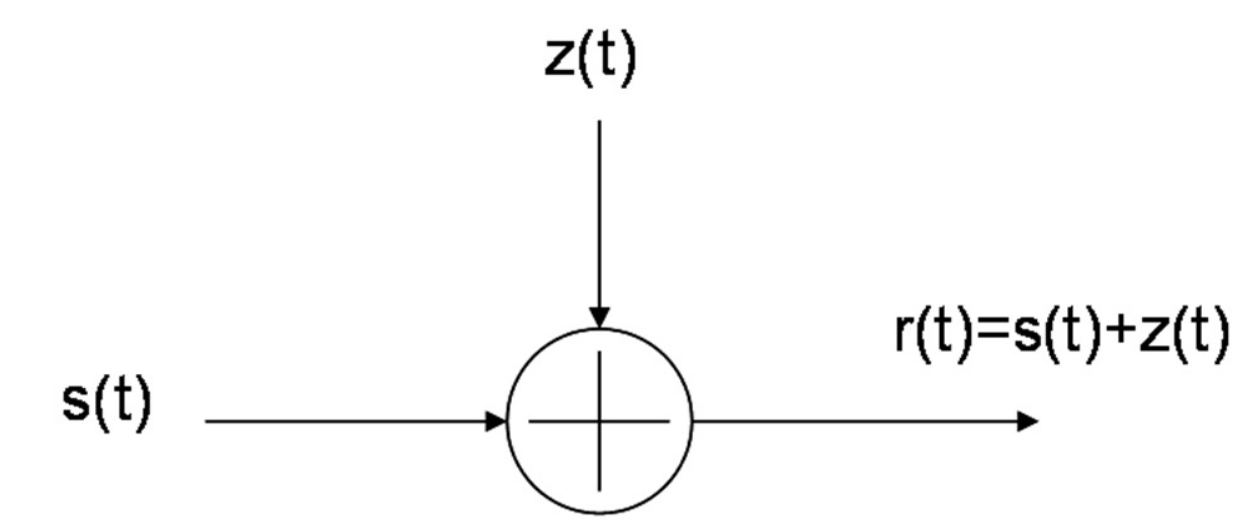
\includegraphics[width=0.5\linewidth]{awgn/awgn.png}
    \caption{Az AWGN csatorna modellje}
    \label{fig:awgn}
\end{figure}
\subsection{Mérési feladatok, mérés menete}
A mérési feladat során az AWGN csatorna jelátviteli jellemzőit vizsgáltuk Matlab Simulink környezetben. A mérés az előre összeállított, \ref{fig:awgnmod}.~ábrán látható AWGN csatornamodell betöltésével kezdődött. A rendszer bemeneti gerjesztését a \texttt{simin} változó biztosította, melynek értékeit \aref{lst:simin}.~programkódban található paranccsal generáltuk.
\begin{lstlisting} [caption={Bemenet generálása}, label={lst:simin}]
simin = mod(round(10*rand(1,100)), 4);
\end{lstlisting}
\begin{figure}[h]
    \centering
    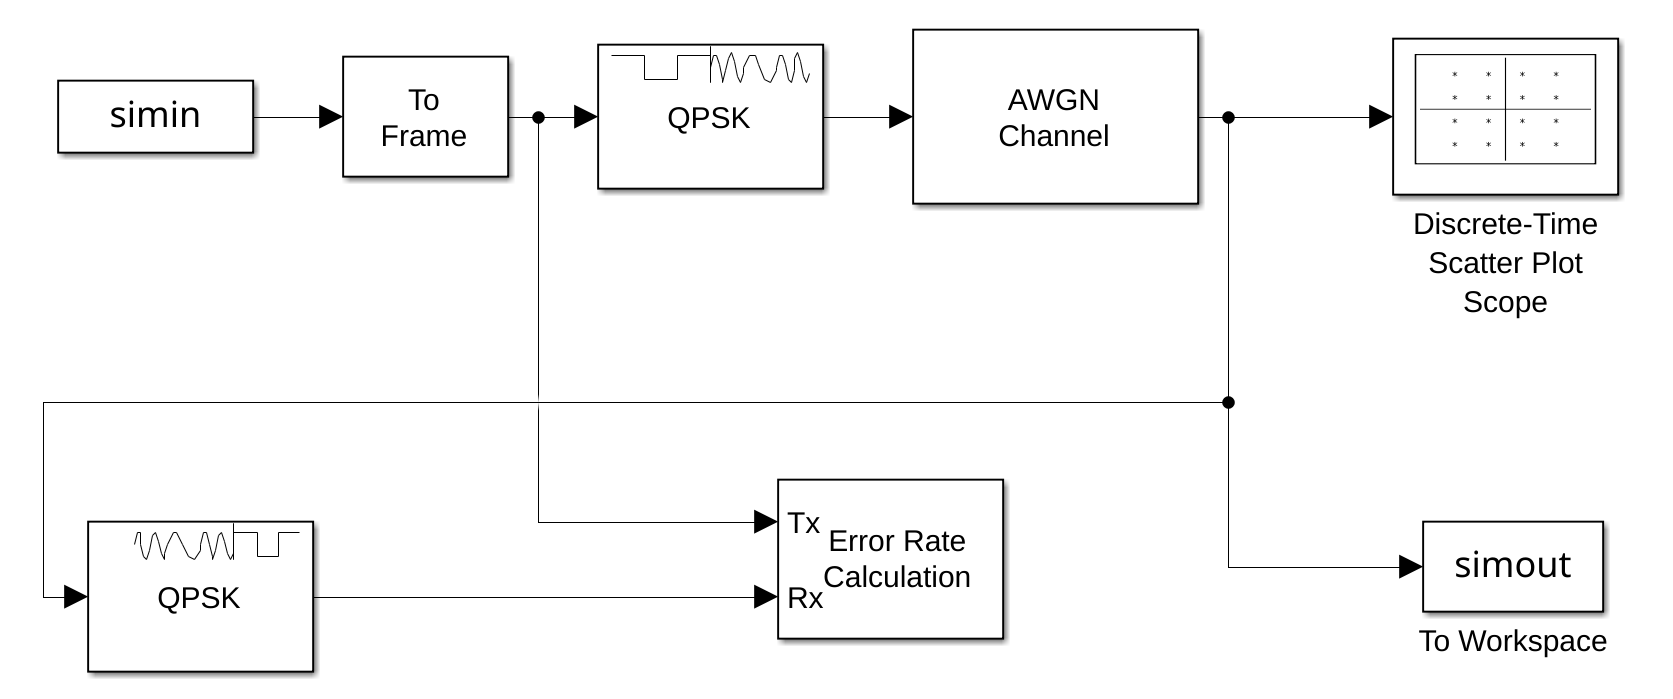
\includegraphics[width=0.7\linewidth]{awgn/awgn_mod.png}
    \caption{A használt AWGN csatornamodell}
    \label{fig:awgnmod}
\end{figure} Ez a parancs 100 darab, véletlenszerűen választott szimbólumot hoz létre a $\{0, 1, 2, 3\}$ halmazból, lehetővé téve a négy állapotú (QPSK) átvitel vizsgálatát. A szimuláció során megfigyelhettük a konstellációs diagram dinamikus változását. A szimulációs időt $t_\text{sim} = 10^{-4}\, \mathrm{s}$ értékre állítottuk be. A futtatást követően a kimeneti jelet \aref{lst:simout}. programkód parancsaival dolgoztuk fel és jelenítettük meg az amplitúdó időbeli eloszlását.
\begin{lstlisting}[caption={Kimenet transzformálása}, label={lst:simout}]
dataout=simout.signals.values; %Simulink kimenet kiolvasasa
ampl=abs(dataout); %amplitudo generalasa az adatokbol
density=densityf(ampl,'on'); %surusegdiagram
\end{lstlisting}
A rendelkezésre álló modellben állítható az egyes csatornablokkok SNR szintje. Ez az adott blokkra kattintva módosítható.
Feladatunk  az átvitel minőségének vizsgálata és az amplitúdó időbeli eloszlásának megjelenítése volt 5, 10 és 15dB SNR értékek mellett.

\begin{figure}[b]
    \centering
    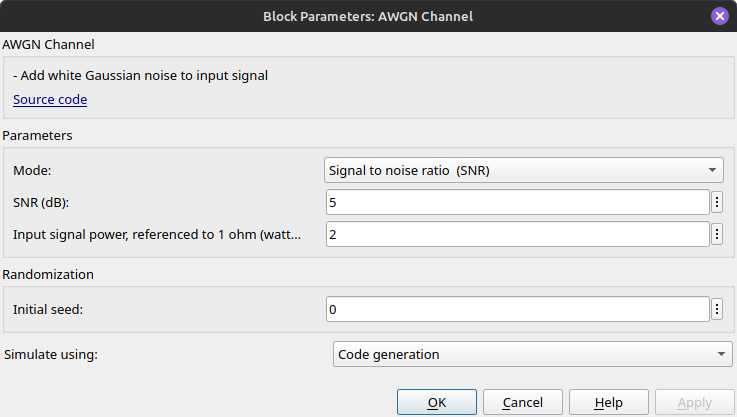
\includegraphics[width=0.5\linewidth]{awgn/awgn_set.png}
    \caption{Az AWGN csatornablokk beállításai}
    \label{fig:awgnset}
\end{figure}

\subsection{Kapott eredmények, értékelés}
A mérés során \aref{fig:awgn_res}.~ábrán látható eredményeket kaptuk.
\begin{figure}[hp]
     \centering
     \begin{subfigure}[b]{0.5\textwidth}
         \centering
         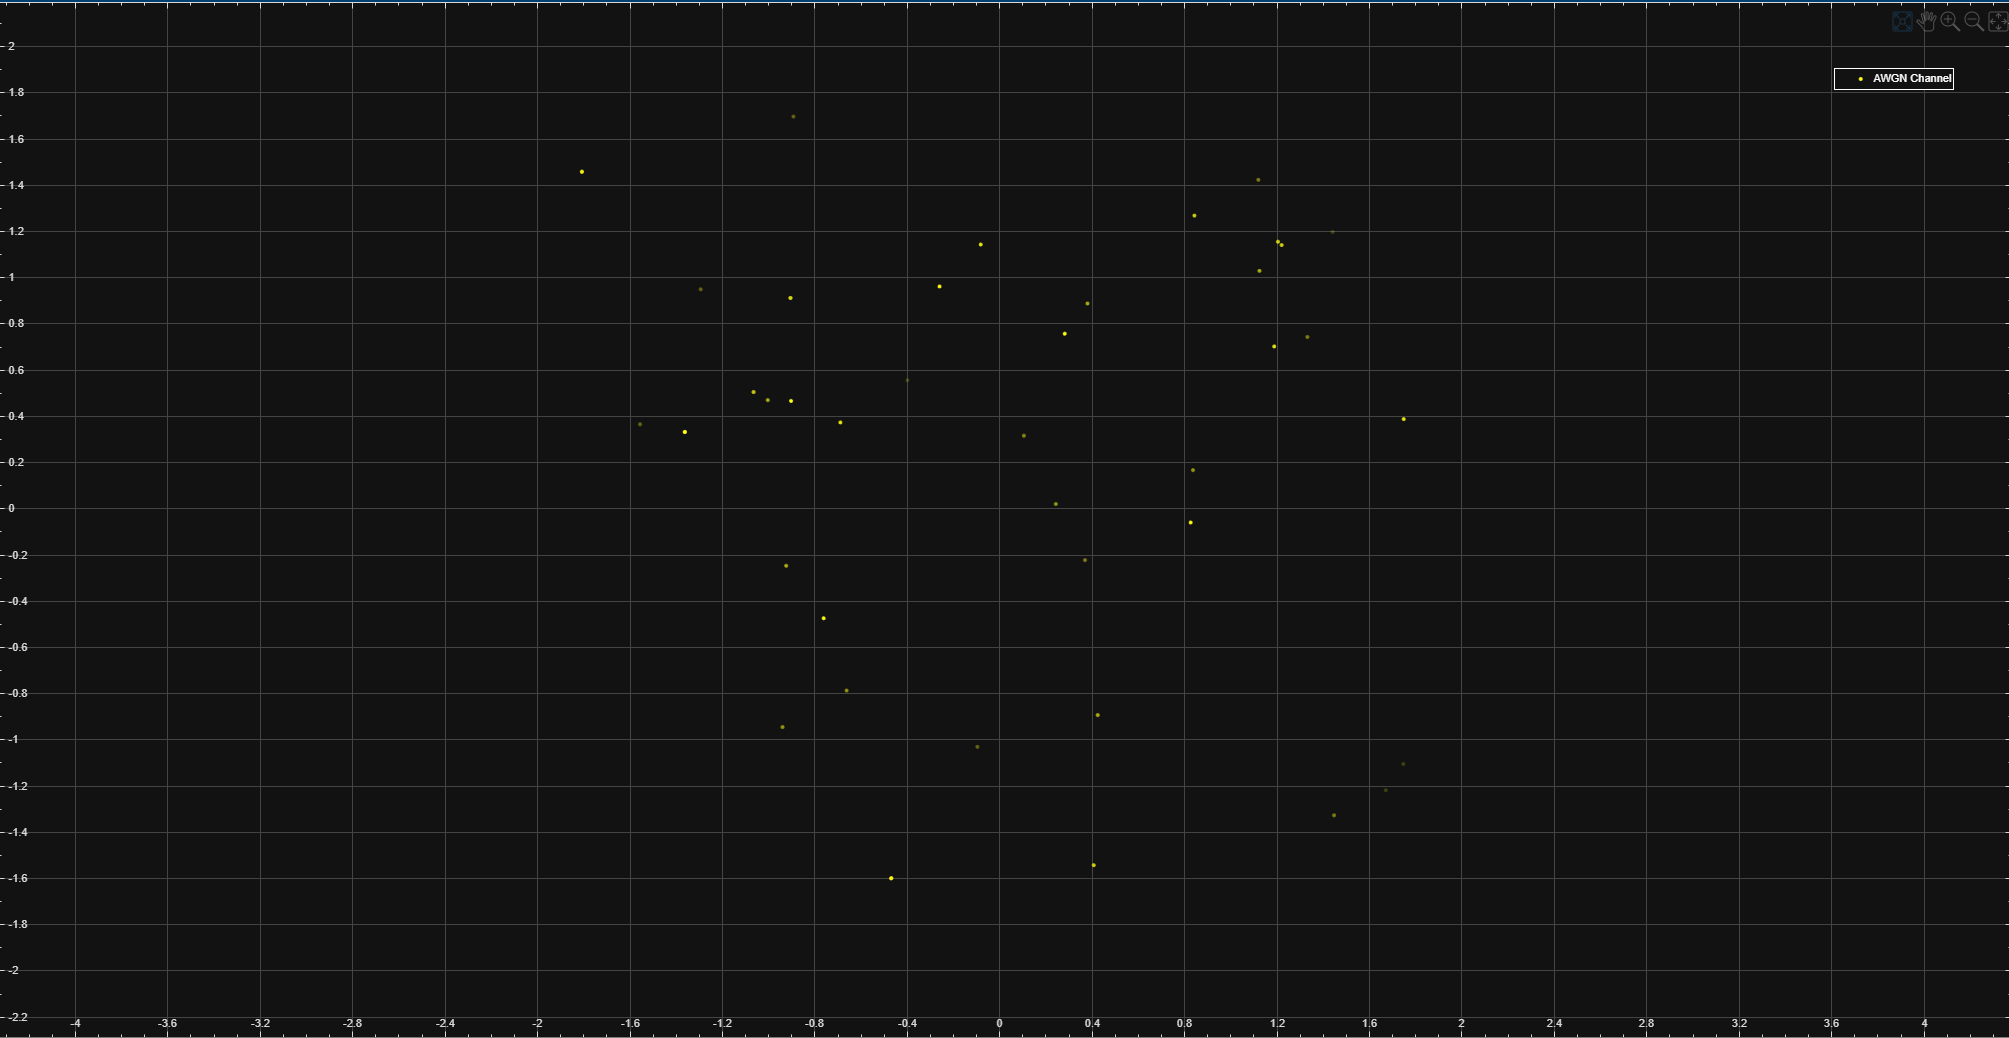
\includegraphics[width=\textwidth]{awgn/awgn5db.png}
         \caption{5 dB-es konstellációs diagram}
         \label{fig:awgn_const5}
     \end{subfigure}
     \hfill
          \begin{subfigure}[b]{0.4\textwidth}
         \centering
         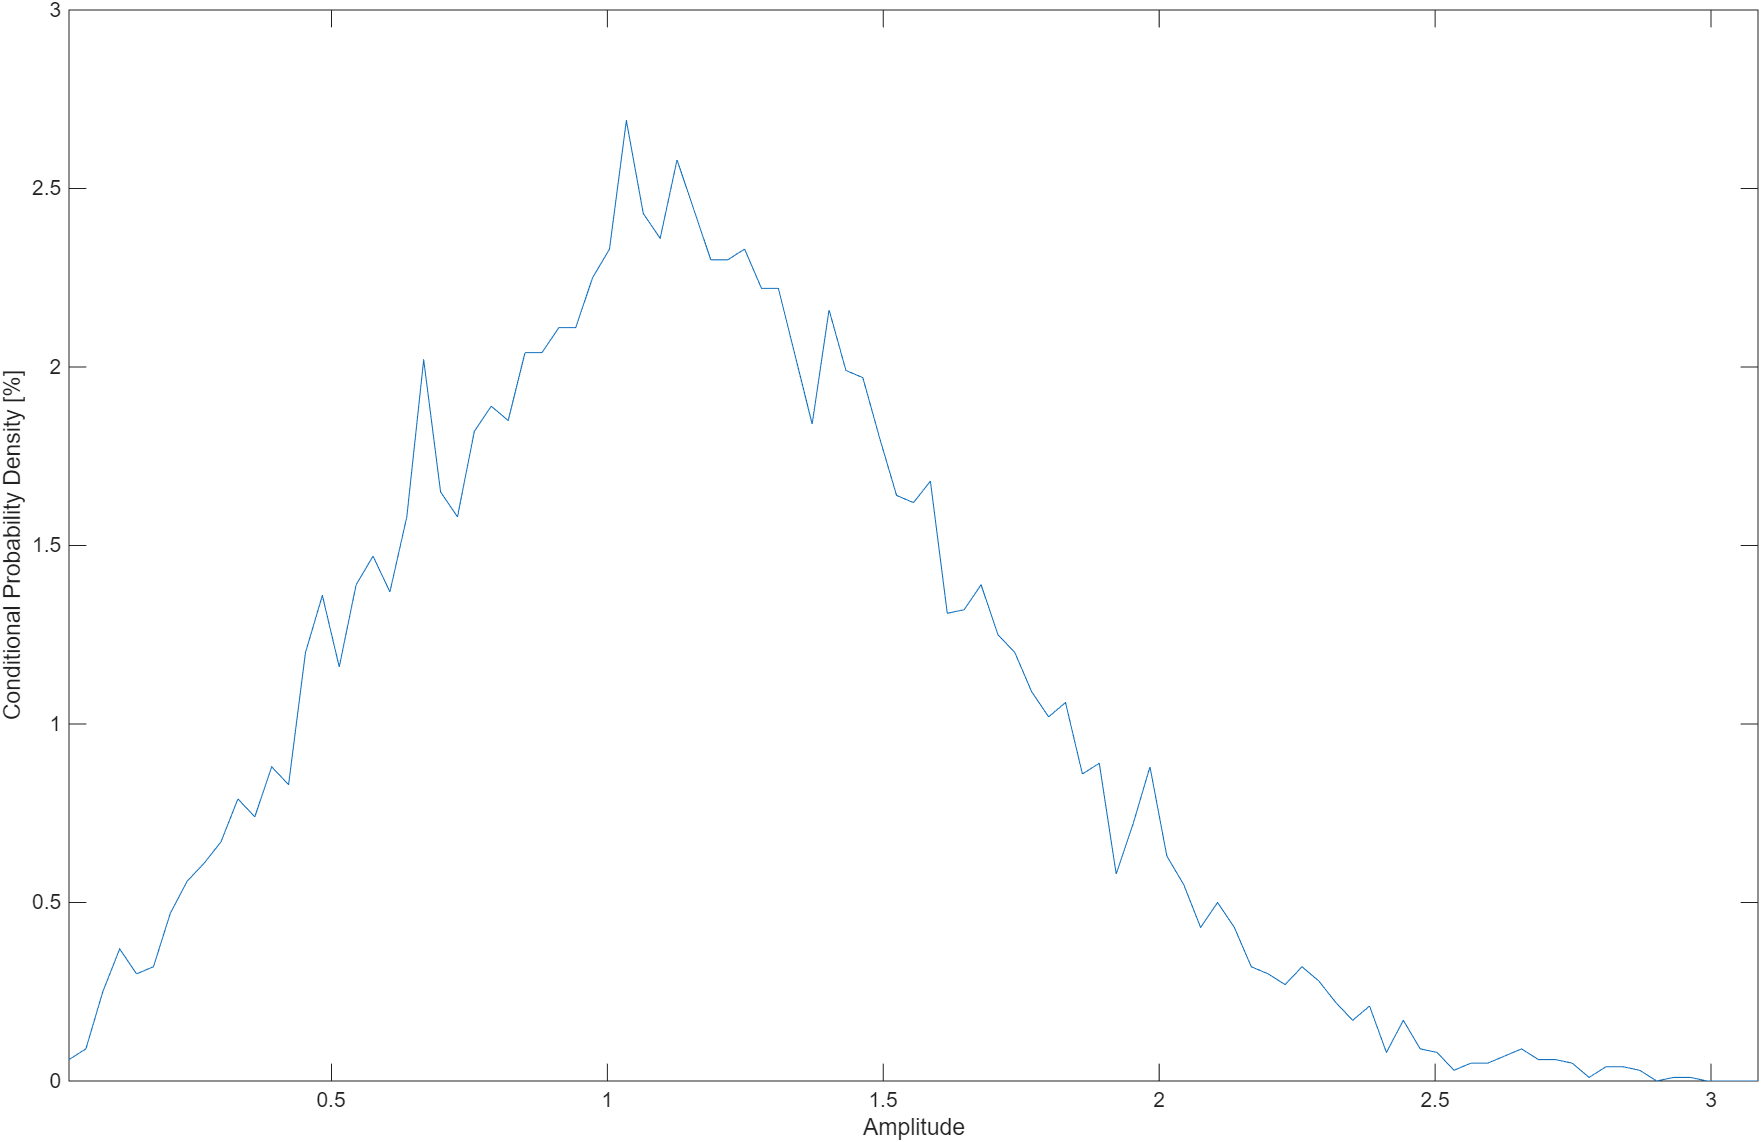
\includegraphics[width=\textwidth]{awgn/awgn5db_d.png}
         \caption{5 dB-es eloszlás}
         \label{fig:awgn_d5}
     \end{subfigure}
     \hfill
     \begin{subfigure}[b]{0.5\textwidth}
         \centering
         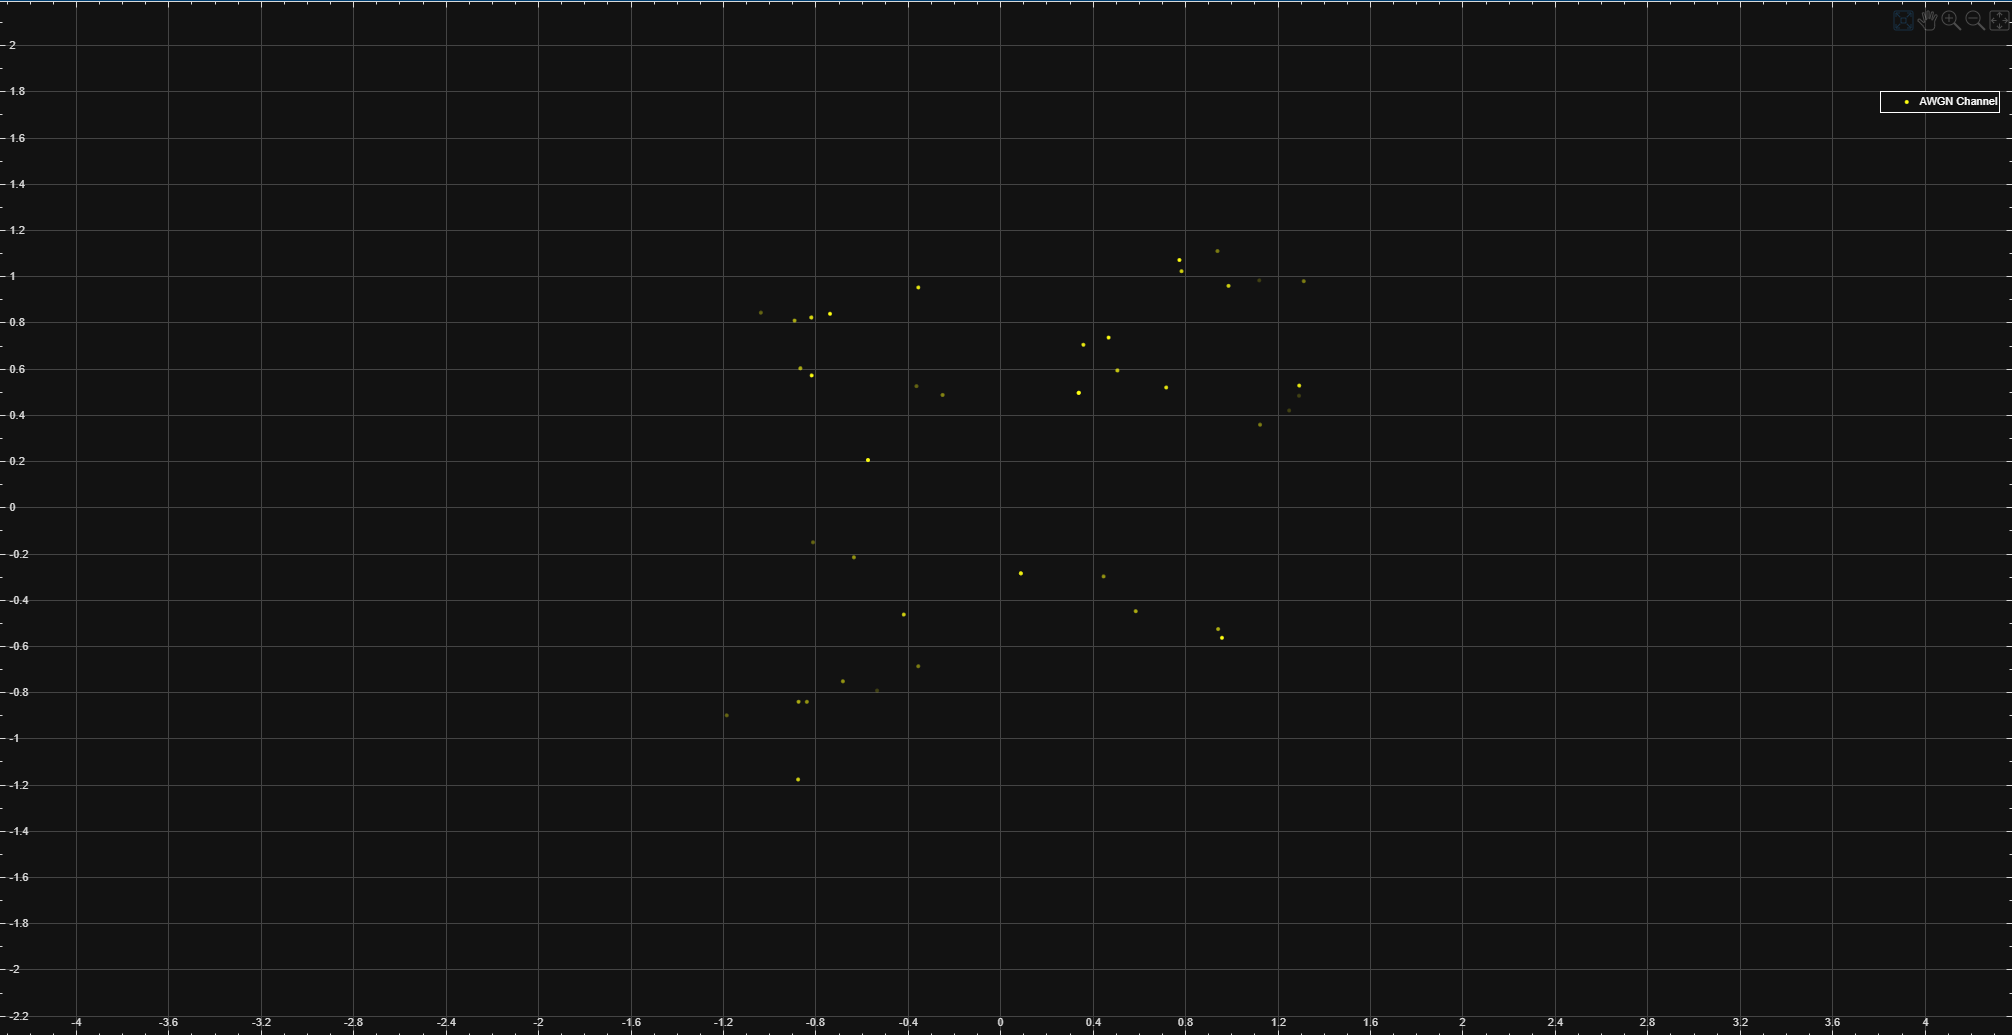
\includegraphics[width=\textwidth]{awgn/awgn10db.png}
         \caption{10 dB-es konstellációs diagram}
         \label{fig:awgn_const10}
     \end{subfigure}
     \hfill
     \begin{subfigure}[b]{0.4\textwidth}
         \centering
         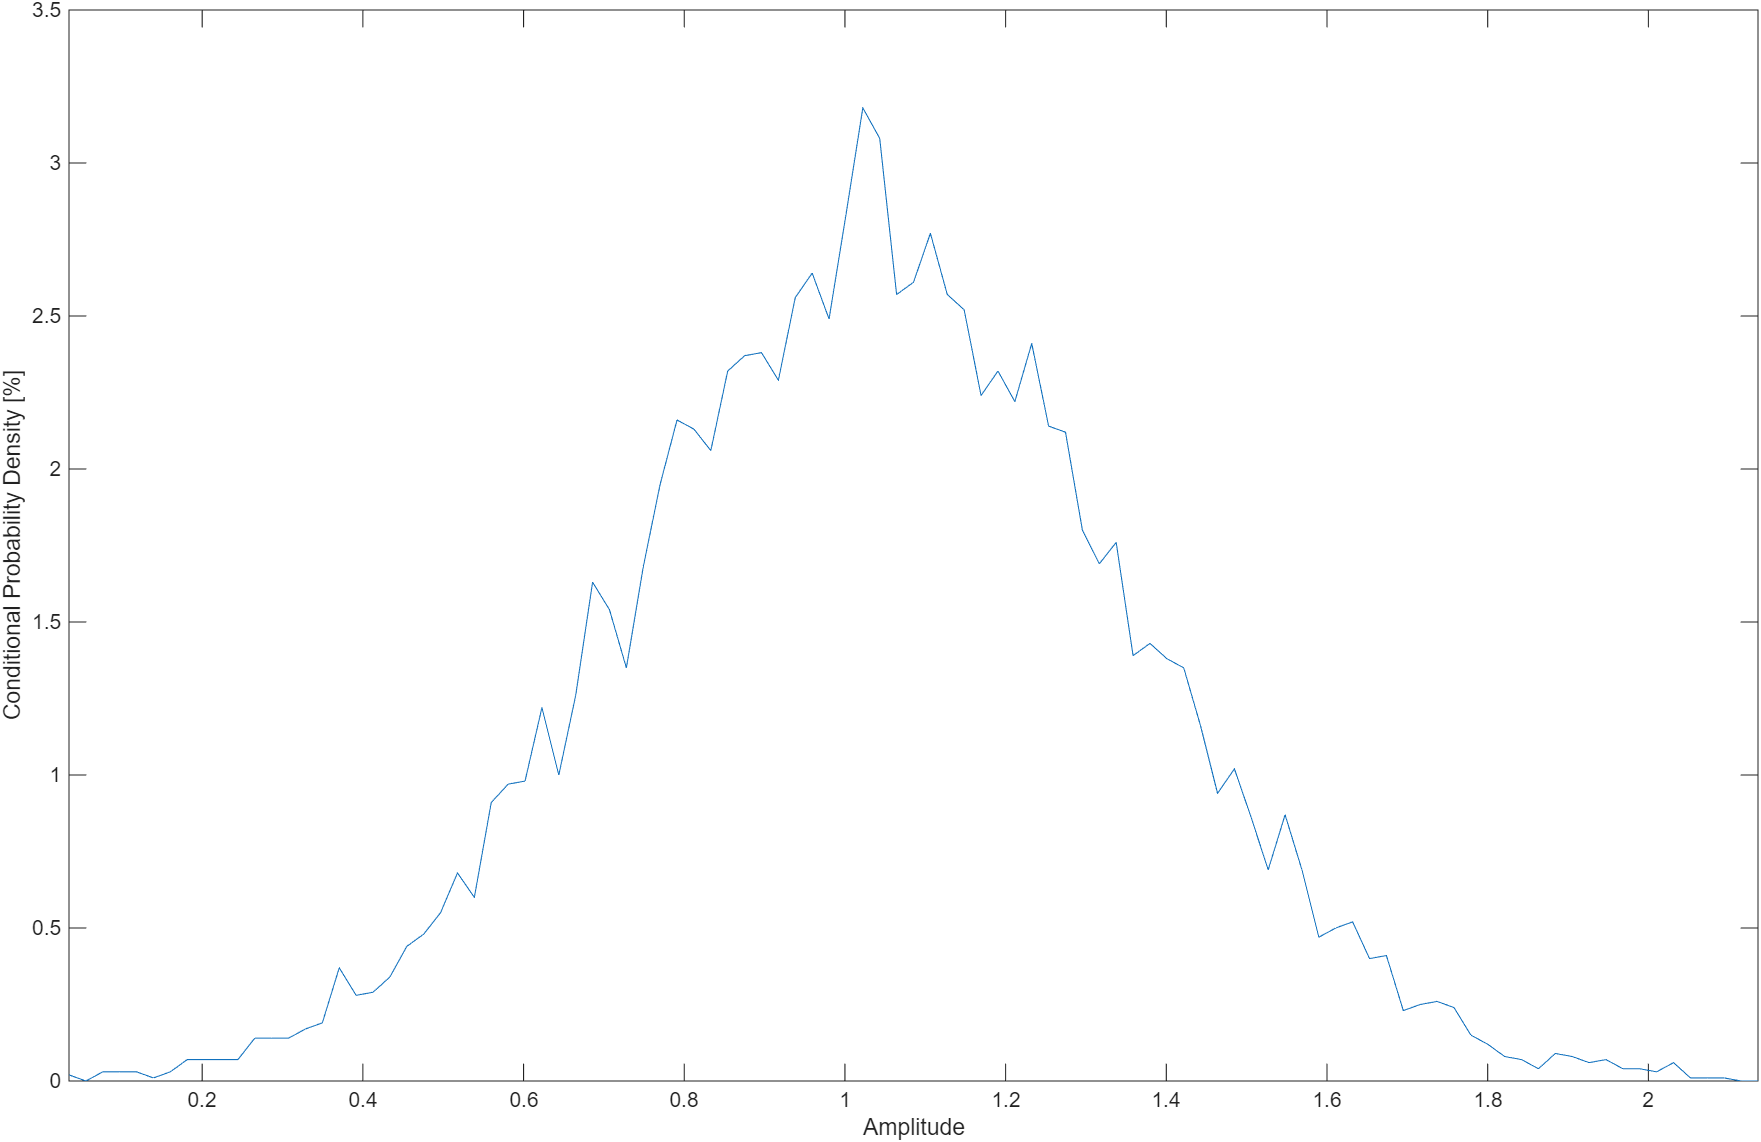
\includegraphics[width=\textwidth]{awgn/awgn10db_d.png}
         \caption{10 dB-es eloszlás}
         \label{fig:awgn_d10}
     \end{subfigure}
     \hfill
          \begin{subfigure}[b]{0.5\textwidth}
         \centering
         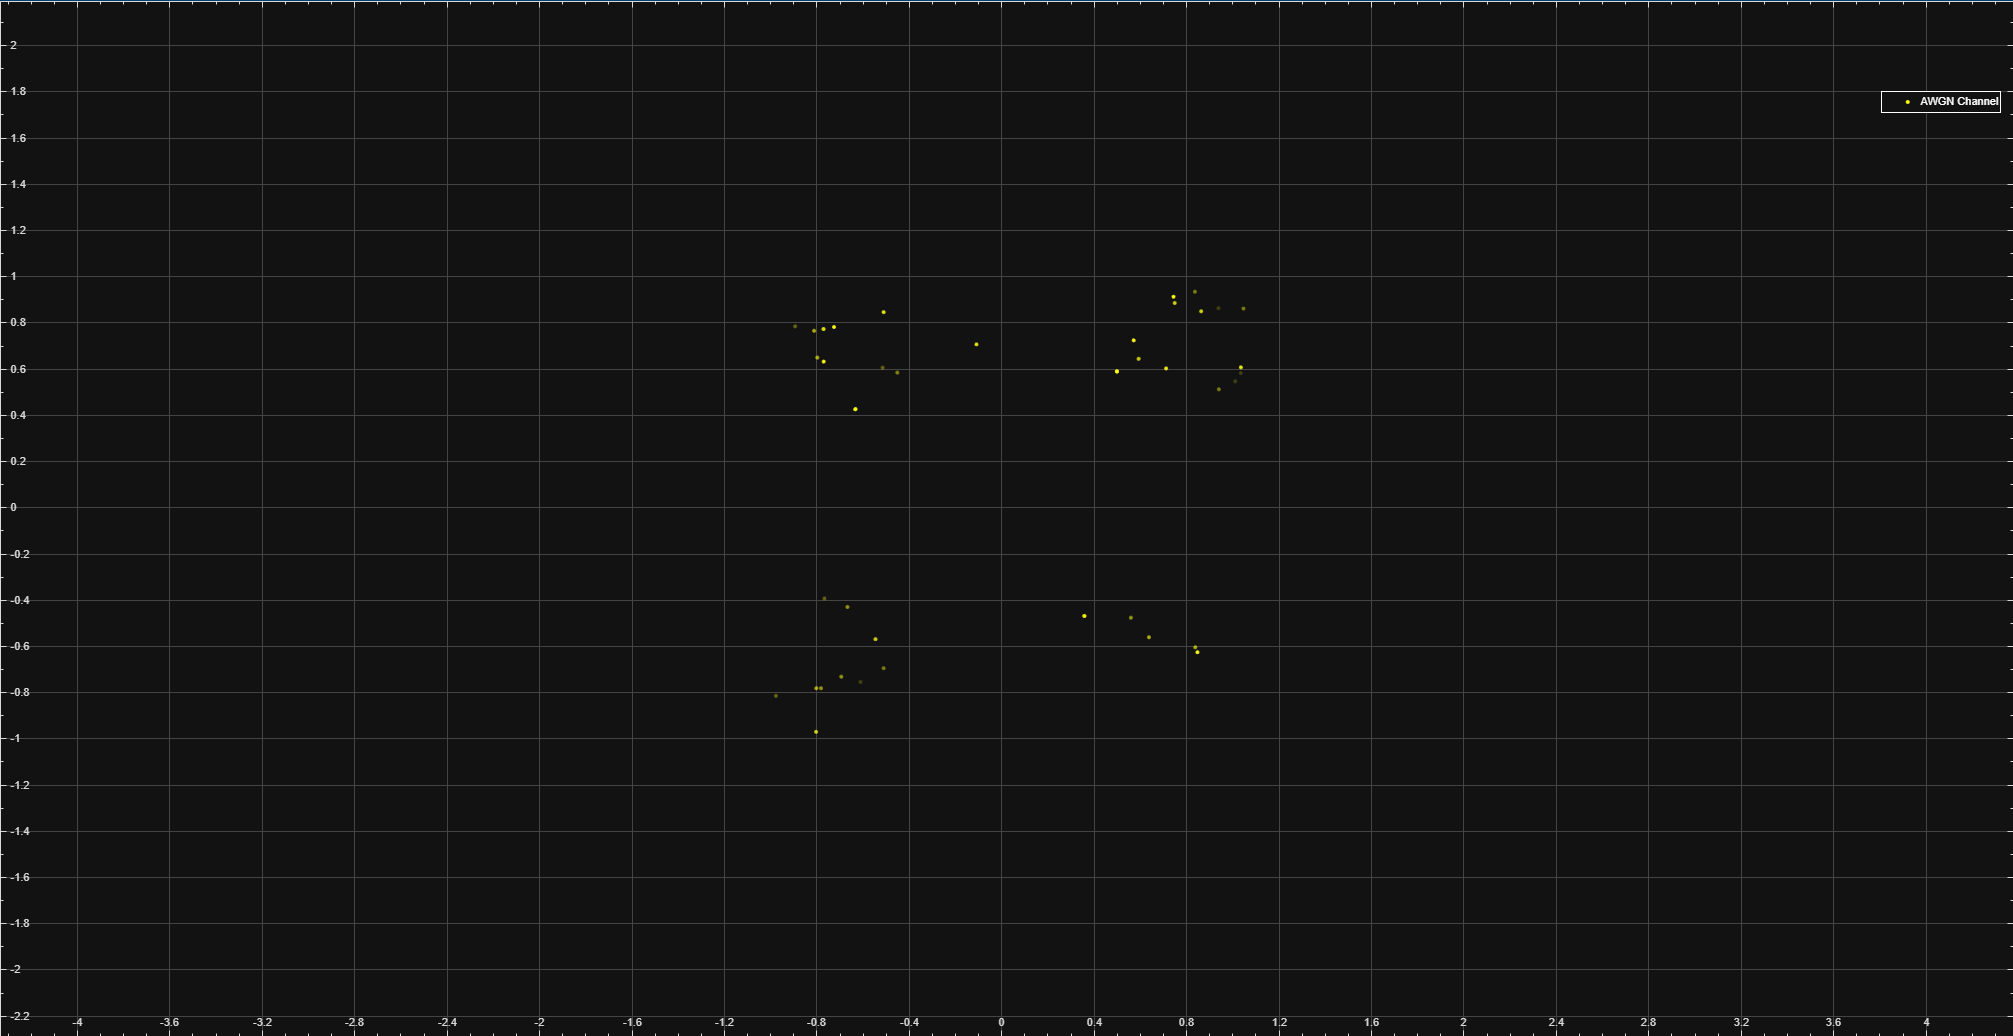
\includegraphics[width=\textwidth]{awgn/awgn15db.png}
         \caption{15 dB-es konstellációs diagram}
         \label{fig:awgn_const15}
     \end{subfigure}
     \hfill
     \begin{subfigure}[b]{0.4\textwidth}
         \centering
         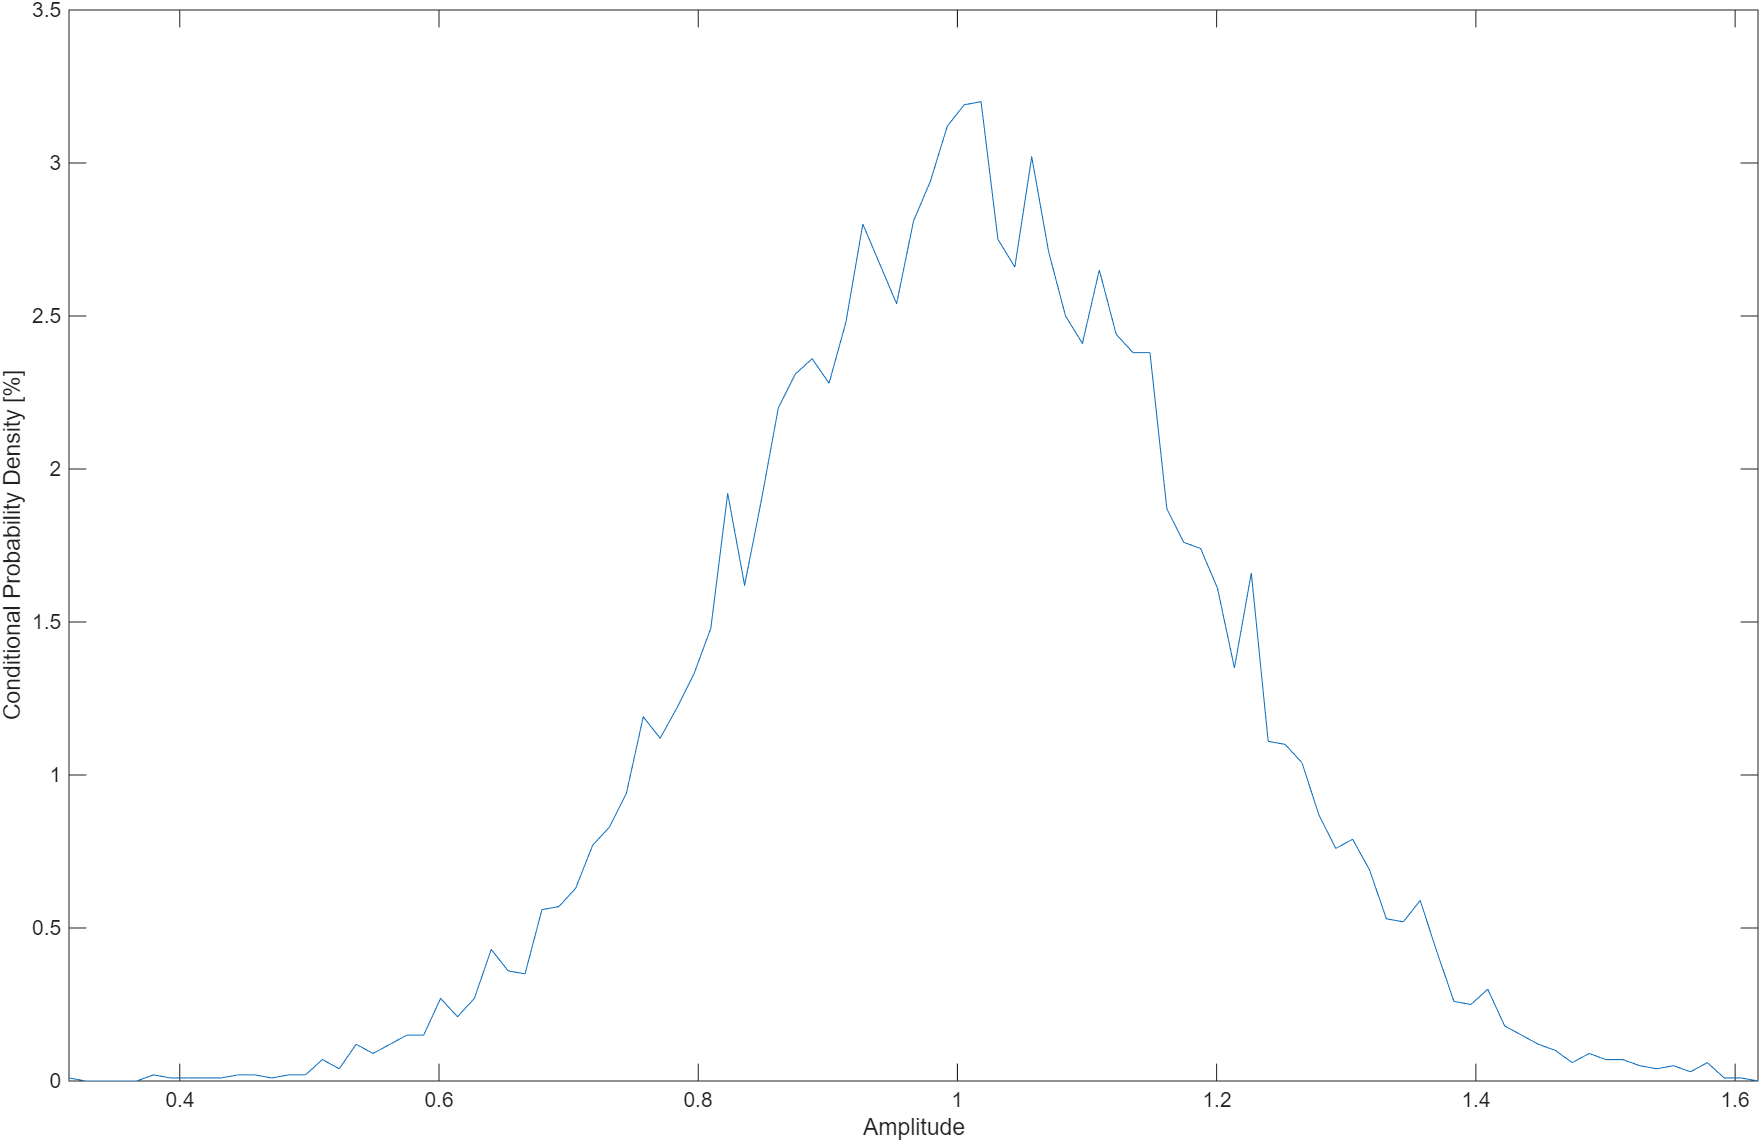
\includegraphics[width=\textwidth]{awgn/awgn15db_d.png}
         \caption{15 dB-es eloszlás}
         \label{fig:awgn_d15}
     \end{subfigure}
        \caption{Az AWGN Csatorna szimuláció konstellációs diagramjai és eloszlásfüggvényei különböző SNR értékek mellett}
        \label{fig:awgn_res}
\end{figure}
Jól látható, hogy az SNR növekedésével javult az átvitel minősége, azaz csökkent a bithiba arány. A konstellációs diagramok is kisebb szóródást mutatnak, valamint az amplitúdó időbeli eloszlásában is kisebb szórás figyelhető meg. Ez magyarázható az SNR növekedésével. A hibaarány kiolvasható a futást követően az  \verb|ErrorVec| változó első sorából. Az egyes SNR értékeket és a hozzájuk tartozó hibaarányt \aref{tab:awgnError}.~táblázat tartalmazza.

\begin{table}
    \centering
    \begin{tabular}{|c|c|c|c|}
      \hline SNR [dB] & 5 & 10 & 15\\\hline
      Hibaarány [\%] & 19,65 & 2,4502 & $1,0001\cdot10^{-4}$\\ \hline
    \end{tabular}
    \caption{Az AWGN Modell egyes SNR értékeihez tartozó hibaarányai}
    \label{tab:awgnError}
\end{table}

\section{Rayleigh csatornamodell}
\subsection{Elméleti háttér}
A mérést a Rayleigh és Rice csatornamodellek vizsgálatával folytattuk, elsőként a Rayleigh modellt elemeztük.
Többutas terjedés esetén a vett $r$ jel a különböző utakról érkező $a_i$ jelek fázishelyes
összegeként adódik. Ez az összegzés elvégezhető külön-külön a vetületekre is, és a különböző utakról érkező jelek vektori összege adja a vett jelet. A Rayleigh csatornamodellt olyan többutas jelterjedési modellezésnél használjuk, amikor az adó és vevő nincsenek közvetlen rálátásra egymásra, valamint a komplex burkoló összetevői Gauss-folyamatok 0 várható értékkel.

% <többutas terjedés diagram, csak ha nagyon sok időm lesz majd xd>


\subsection{Mérési feladatok, mérés menete}
A Rayleigh csatornamodell vizsgálatánál hasonlóan jártunk el, mint AWGN esetben. A Simulink Rayleigh csatornamodell \aref{fig:raymod}.~ábrán látható.
\begin{figure}[h]
    \centering
    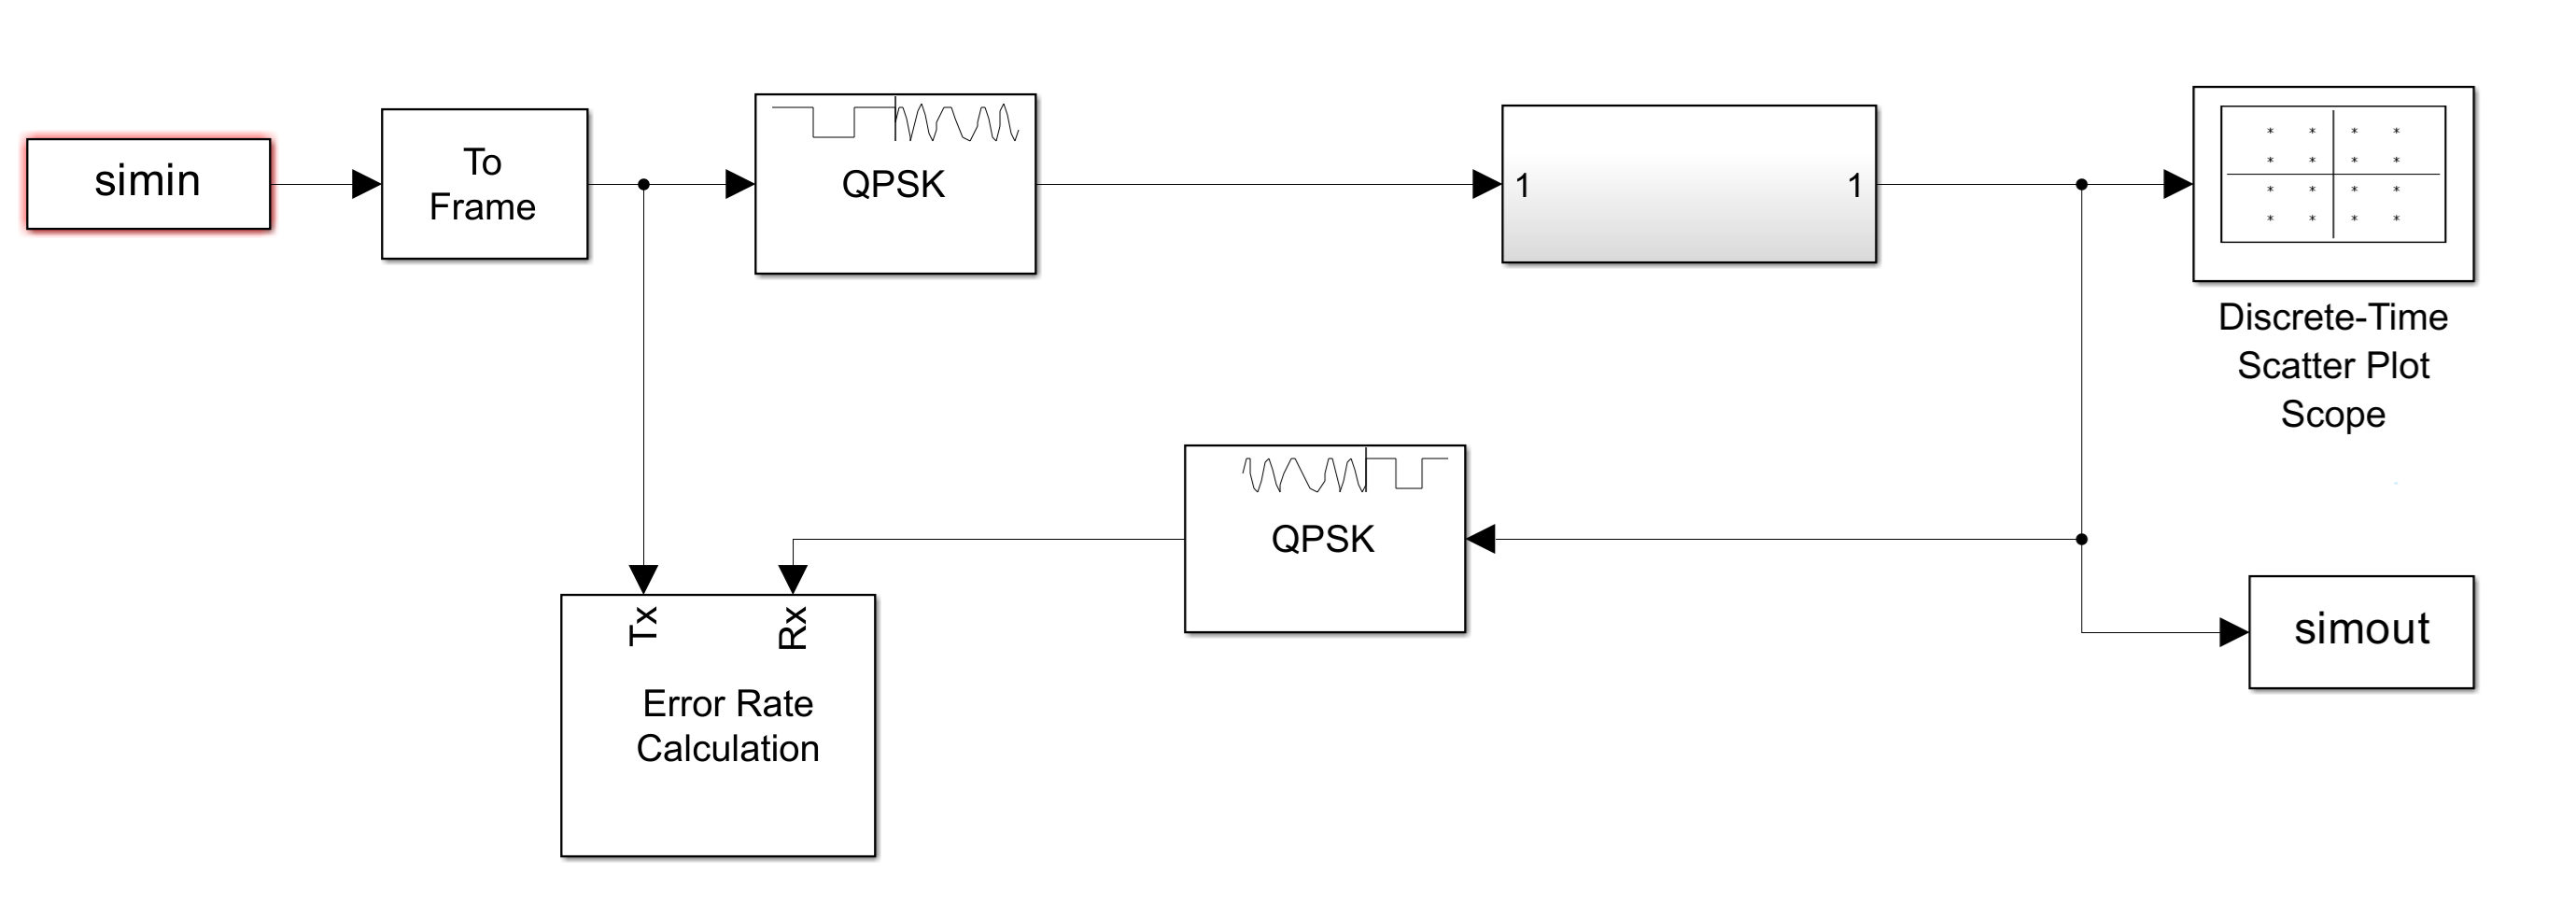
\includegraphics[width=0.7\linewidth]{ray/ray_mod.png}
    \caption{A használt Rayleigh csatornamodell}
    \label{fig:raymod}
\end{figure} Lényeges különbség az AWGN modellhez képest, hogy itt a csatornablokkban nem közvetlen SNR értéket állítottunk be. A csatorna minőségét a fázis- és amplitúdószórás paramétereinek változtatásával (azaz a Gauss-folyamatok varianciájának módosításával) szabályoztuk.

\begin{figure}[hp]
     \centering
     \begin{subfigure}[b]{0.4\textwidth}
         \centering
         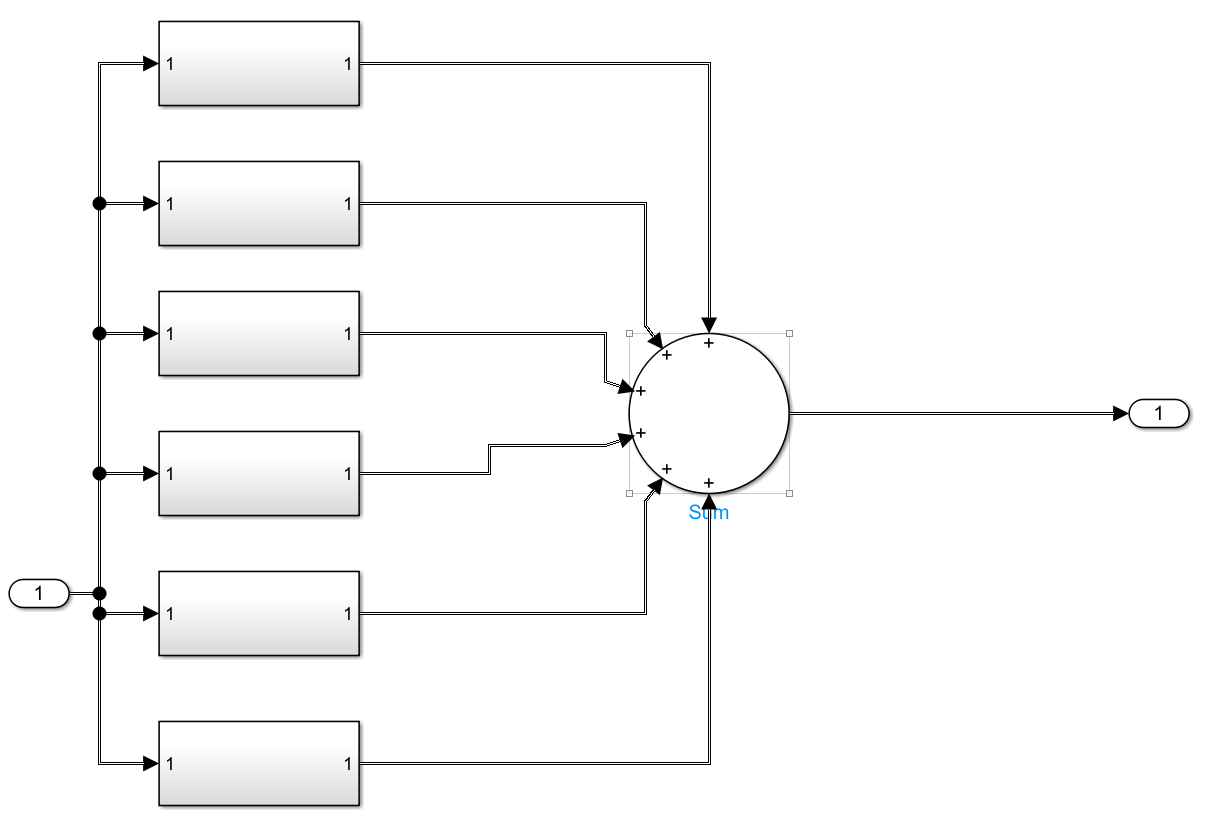
\includegraphics[width=\textwidth]{ray/ray_set1.png}
         \caption{A többutas terjedés megvalósítása}
         \label{fig:ray_set_multpath}
     \end{subfigure}
     \hfill
          \begin{subfigure}[b]{0.55\textwidth}
         \centering
         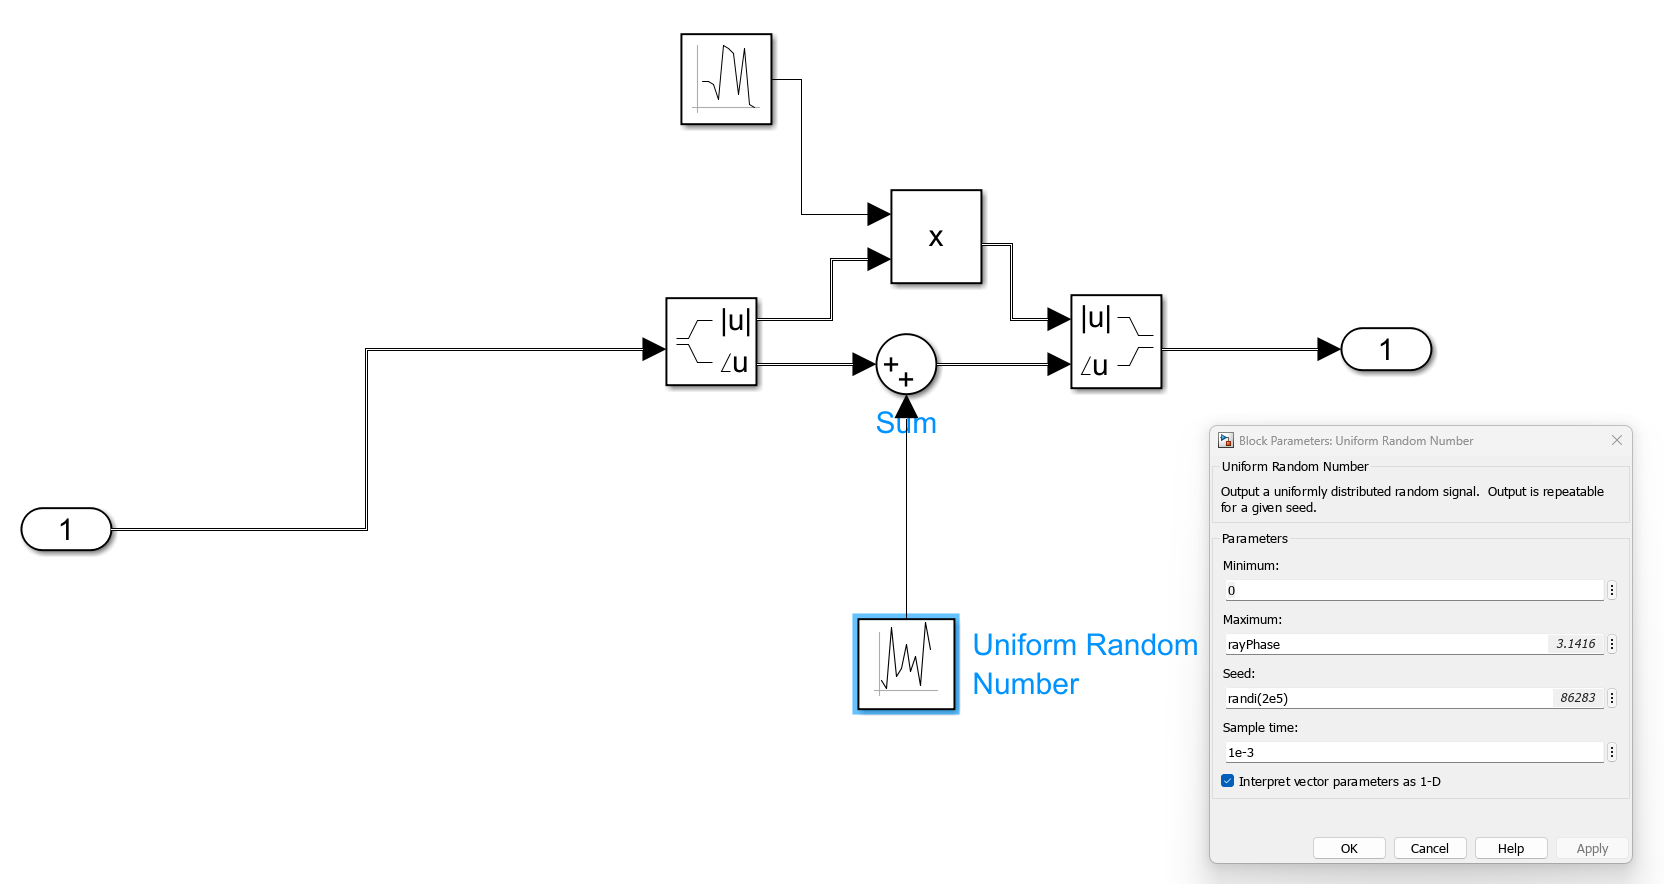
\includegraphics[width=\textwidth]{ray/ray_set2.png}
         \caption{Az egy útra vonatkozó fázistolást a \texttt{rayPhase} változó befolyásolja}
         \label{fig:ray_set_phase}
     \end{subfigure}
        \caption{A szimulációs modell belső felépítése}
        \label{fig:ray_set}
\end{figure}
Minél nagyobb a szórás, annál nagyobb lesz a hibaarány az átvitel során. A mérés során a csatornaparaméterek hangolásával két szélsőséges állapotot hoztunk létre: egy alacsony hibaarányú átvitelt, valamint egy magas hibaarányút. Feladatunk ezen szélsőséges esetek összehasonlító elemzése volt.

\subsection{Kapott eredmények, értékelés}

\begin{figure}[hb]
     \centering
     \begin{subfigure}[b]{0.5\textwidth}
         \centering
         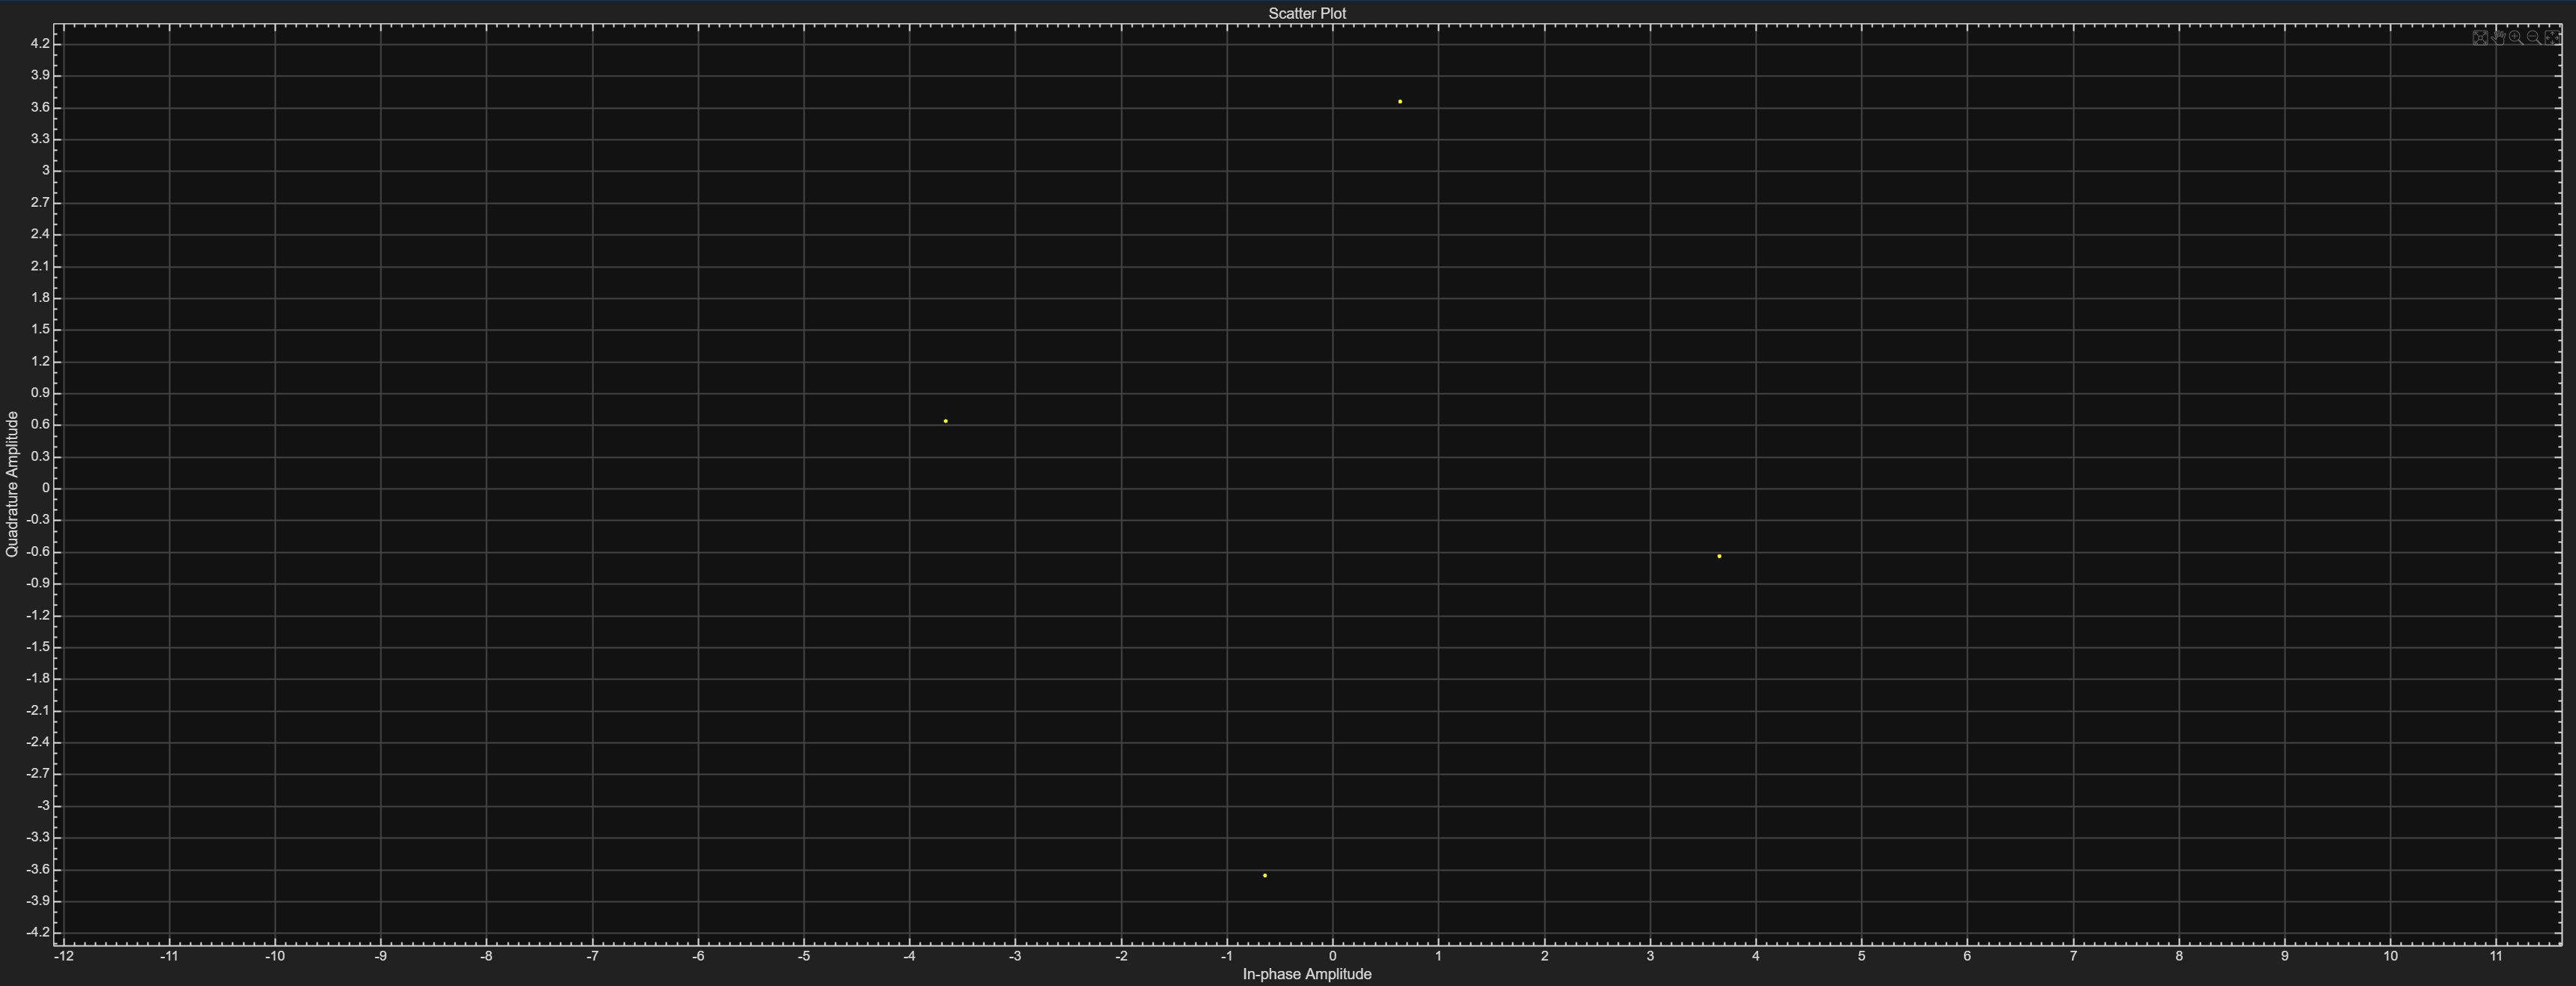
\includegraphics[width=\textwidth]{ray/rayconstpip3.png}
         \caption{$\frac\pi 3$ maximális fázistolású konstellációs diagram}
         \label{fig:ray_const3}
     \end{subfigure}
     \hfill
          \begin{subfigure}[b]{0.4\textwidth}
         \centering
         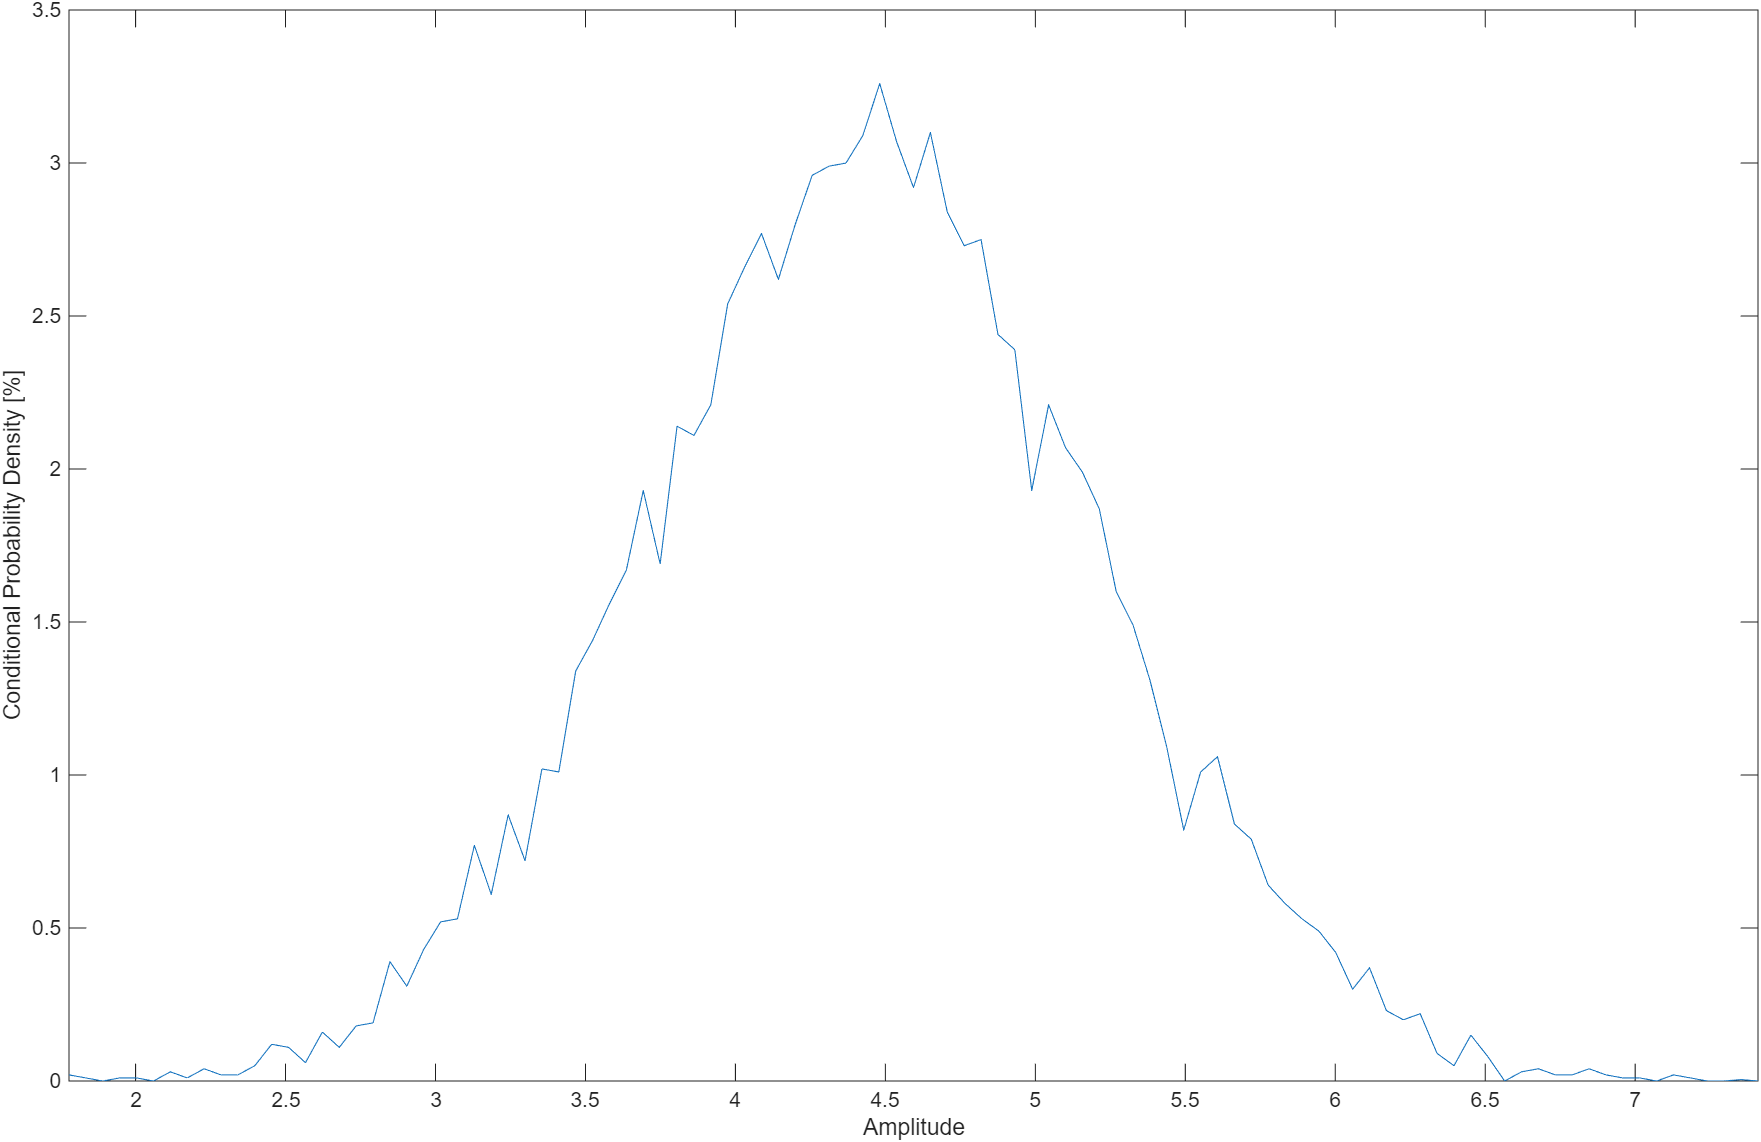
\includegraphics[width=\textwidth]{ray/raydpip3.png}
         \caption{$\frac\pi 3$ maximális fázistolású eloszlás}
         \label{fig:ray_d3}
     \end{subfigure}
     \hfill
     \begin{subfigure}[b]{0.5\textwidth}
         \centering
         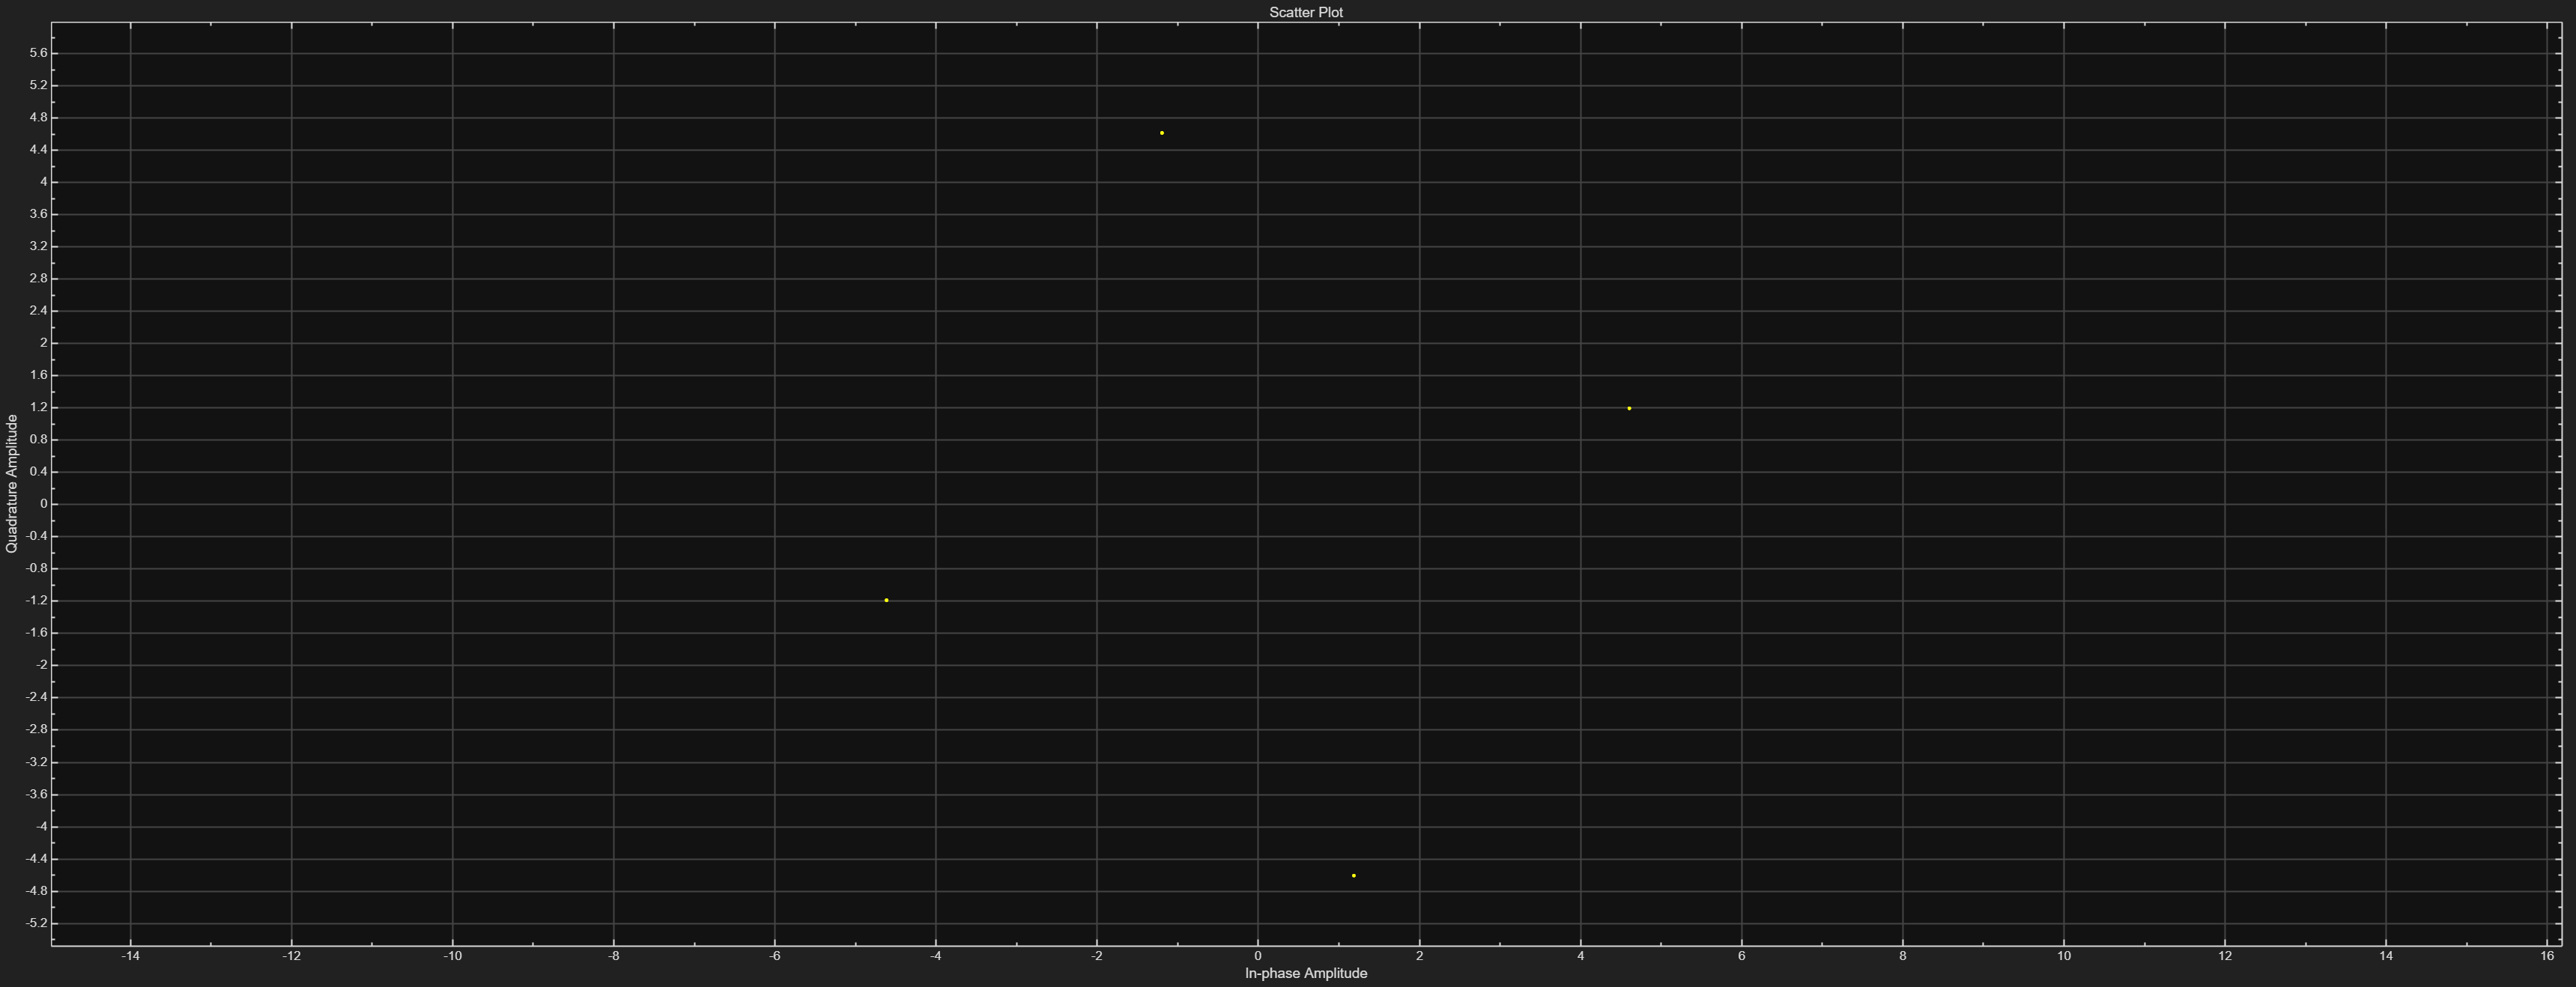
\includegraphics[width=\textwidth]{ray/rayconstpip2.png}
         \caption{$\frac\pi 2$ maximális fázistolású konstellációs diagram}
         \label{fig:ray_const2}
     \end{subfigure}
     \hfill
     \begin{subfigure}[b]{0.4\textwidth}
         \centering
         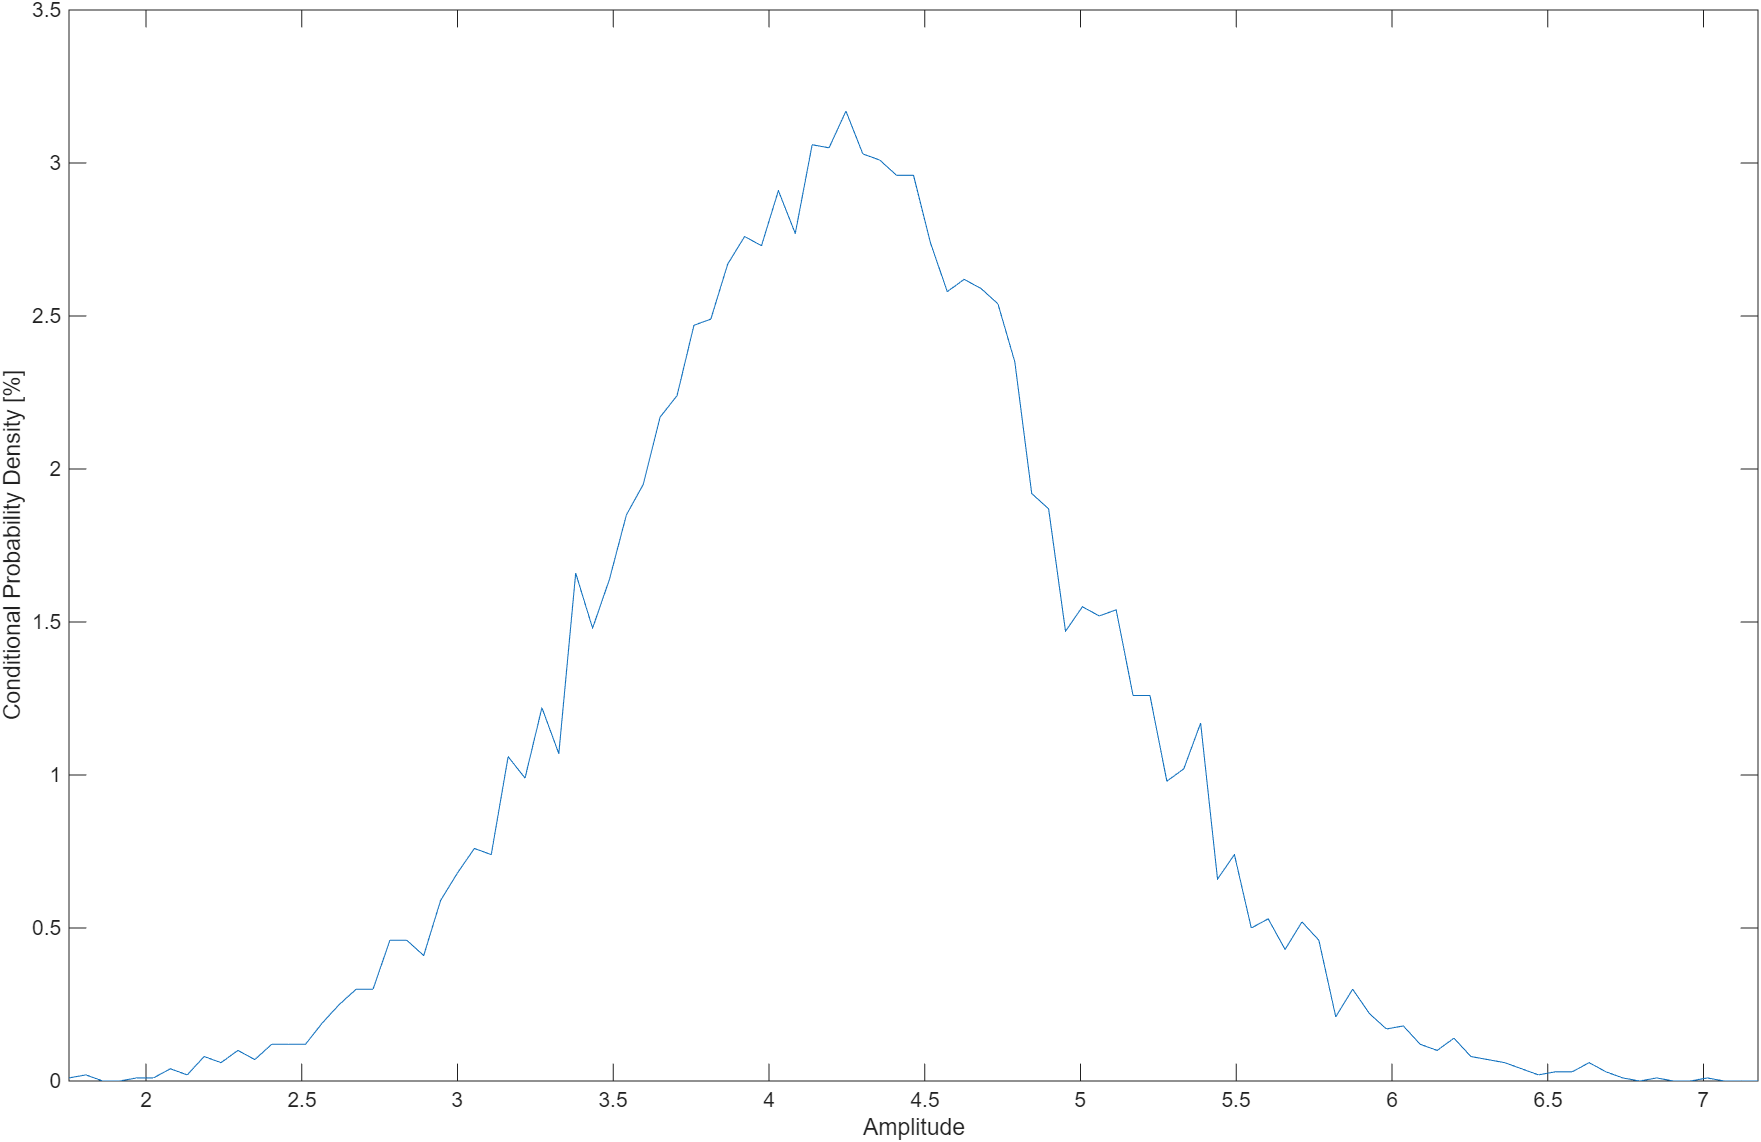
\includegraphics[width=\textwidth]{ray/raydpip2.png}
         \caption{$\frac\pi 2$ maximális fázistolású eloszlás}
         \label{fig:ray_d2}
     \end{subfigure}
        \caption{A Rayleigh Csatorna szimuláció konstellációs diagramjai és eloszlásfüggvényei különböző maximális fázistolások mellett}
        \label{fig:ray_res}
\end{figure}

\begin{table}[hb]
    \centering
    \begin{tabular}{|c|c|c|}
      \hline $\phi_\text{max}$ & $\pi/3$ & ${\pi}/2$\\\hline
      Hibaarány [\%] & 2,70 & 50,29 \\ \hline
    \end{tabular}
    \caption{A Rayleigh Modell különböző maximális fázistolásokhoz tartozó hibaarányai}
    \label{tab:rayError}
\end{table}
A kapott eredményekből jól látható, hogy a fázishiba szórásának növelése drasztikus romlást idézett elő az átvitel minőségében. QPSK moduláció alkalmazásakor a szomszédos konstellációs pontok közötti fázistávolság $90^\circ$, a döntési küszöbök pedig az ideális pontoktól $\pm 45^\circ$-ra helyezkednek el. A mérés során tapasztalt $\phi_\text{max} = \frac\pi2$ fázistolás esetén a kapott 50,29\%-os hibaarány azt jelenti, hogy a vevőoldalon a biteknek több mint a fele hibásan detektálódik. Ekkora hiba mellett érdemi kommunikációt nem lehet megvalósítani az adó és vevő között, ekkora mértékű fázisbizonytalanság nem korrigálható. Ezzel szemben a $\frac\pi3$ fázistolásnál mért 2,7\%-os érték még elfogadható szintet képviselhet, hibajavító kódolással kezelhető, hiszen ekkor 100 elküldött bitből nagyjából 3 lesz hibás. Jól látható, hogy az amplitúdó időbeli eloszlása a két esetben megegyezik. Ez azzal magyarázható, hogy az átvitel romlását csak és kizárólag a fázishiba szórásának manipulálása idézte elő.
\section{Rice csatornamodell}
\subsection{Elméleti háttér}
A Rayleigh modell után a Rice csatornamodellt vizsgáltuk. A Rice csatornamodellt -- a Rayleigh modellhez hasonlóan -- szintén többutas jelterjedés esetén használjuk, amikor az adó és vevőantenna közvetlenül látja egymást (LOS) a komplex burkoló összetevői továbbra is Gauss-folyamatok, de a várható érték nem 0, hanem a közvetlen úton érkező jel.

\begin{figure}[ht]
    \centering
    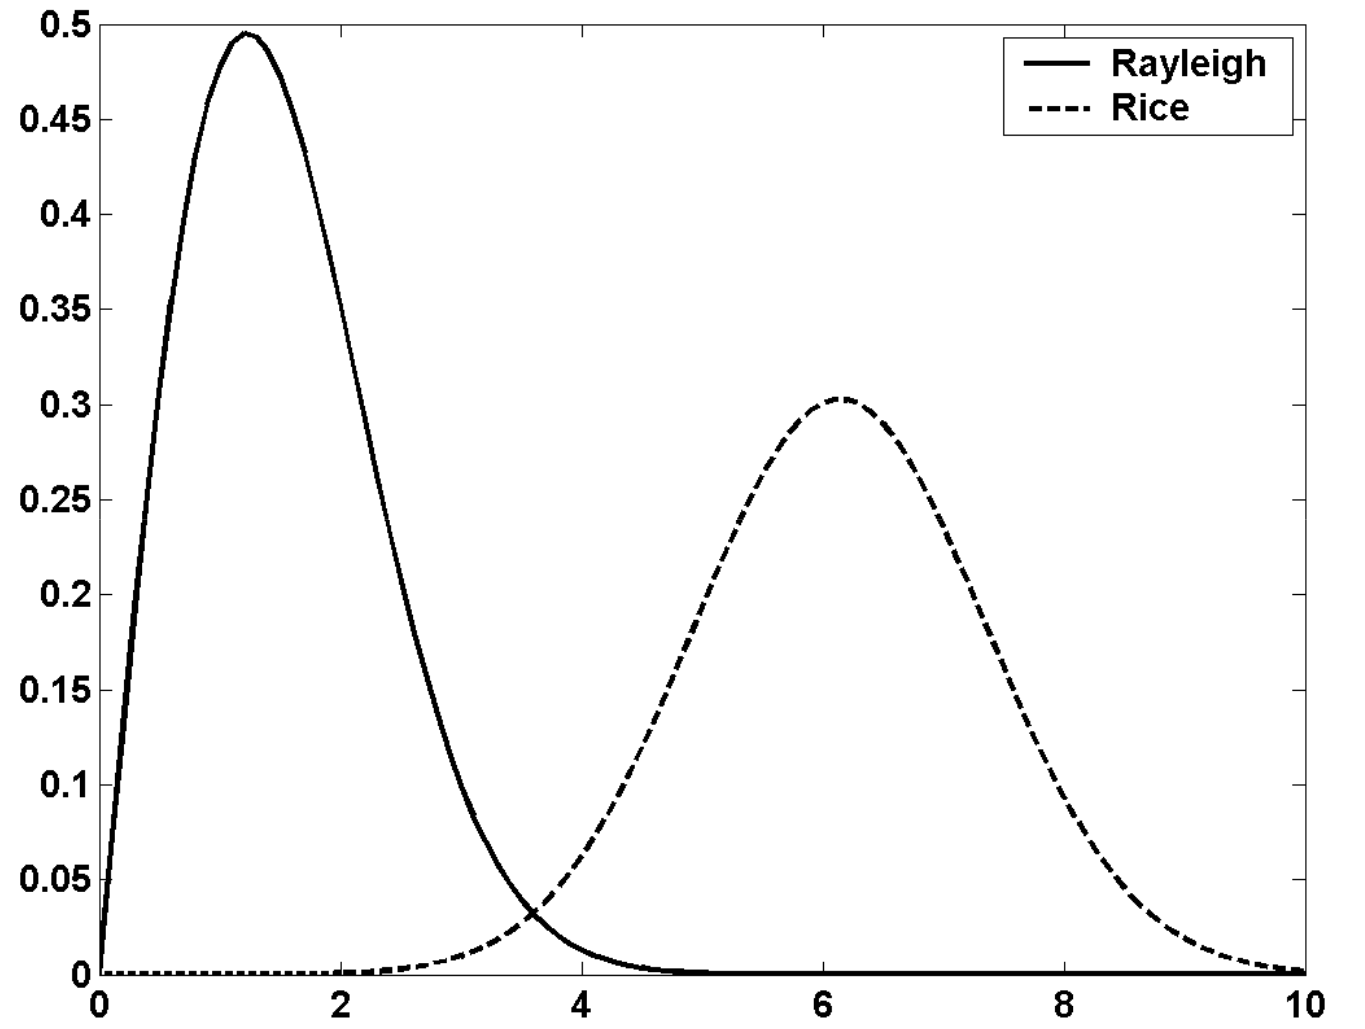
\includegraphics[width=0.4\linewidth]{ray/ray_ric.png}
    \caption{A Rayleigh és Rice modellek elméleti eloszlásai}
    \label{fig:ray_ric}
\end{figure}


\subsection{Mérési feladatok, mérés menete}
A Rice-csatornamodell vizsgálata során a Rayleigh-modellnél megismert mérési lépéseket követtük. A szimuláció célja itt is az átvitel minőségének elemzése volt különböző paraméterbeállítások mellett. Az átvitel minőségének ,,hangolása'' itt is hasonlóan lehetséges, mint a Rayleigh modell esetén, azonban itt az utolsó csatornablokknál nem tudtunk fázisszórást állítani,mivel az elméletben tanultakkal összhangban ez a blokk reprezentálja a közvetlen úton érkező jelösszetevőt.

\subsection{Kapott eredmények, értékelés}

\begin{figure}[htb]
     \centering
     \begin{subfigure}[b]{0.5\textwidth}
         \centering
         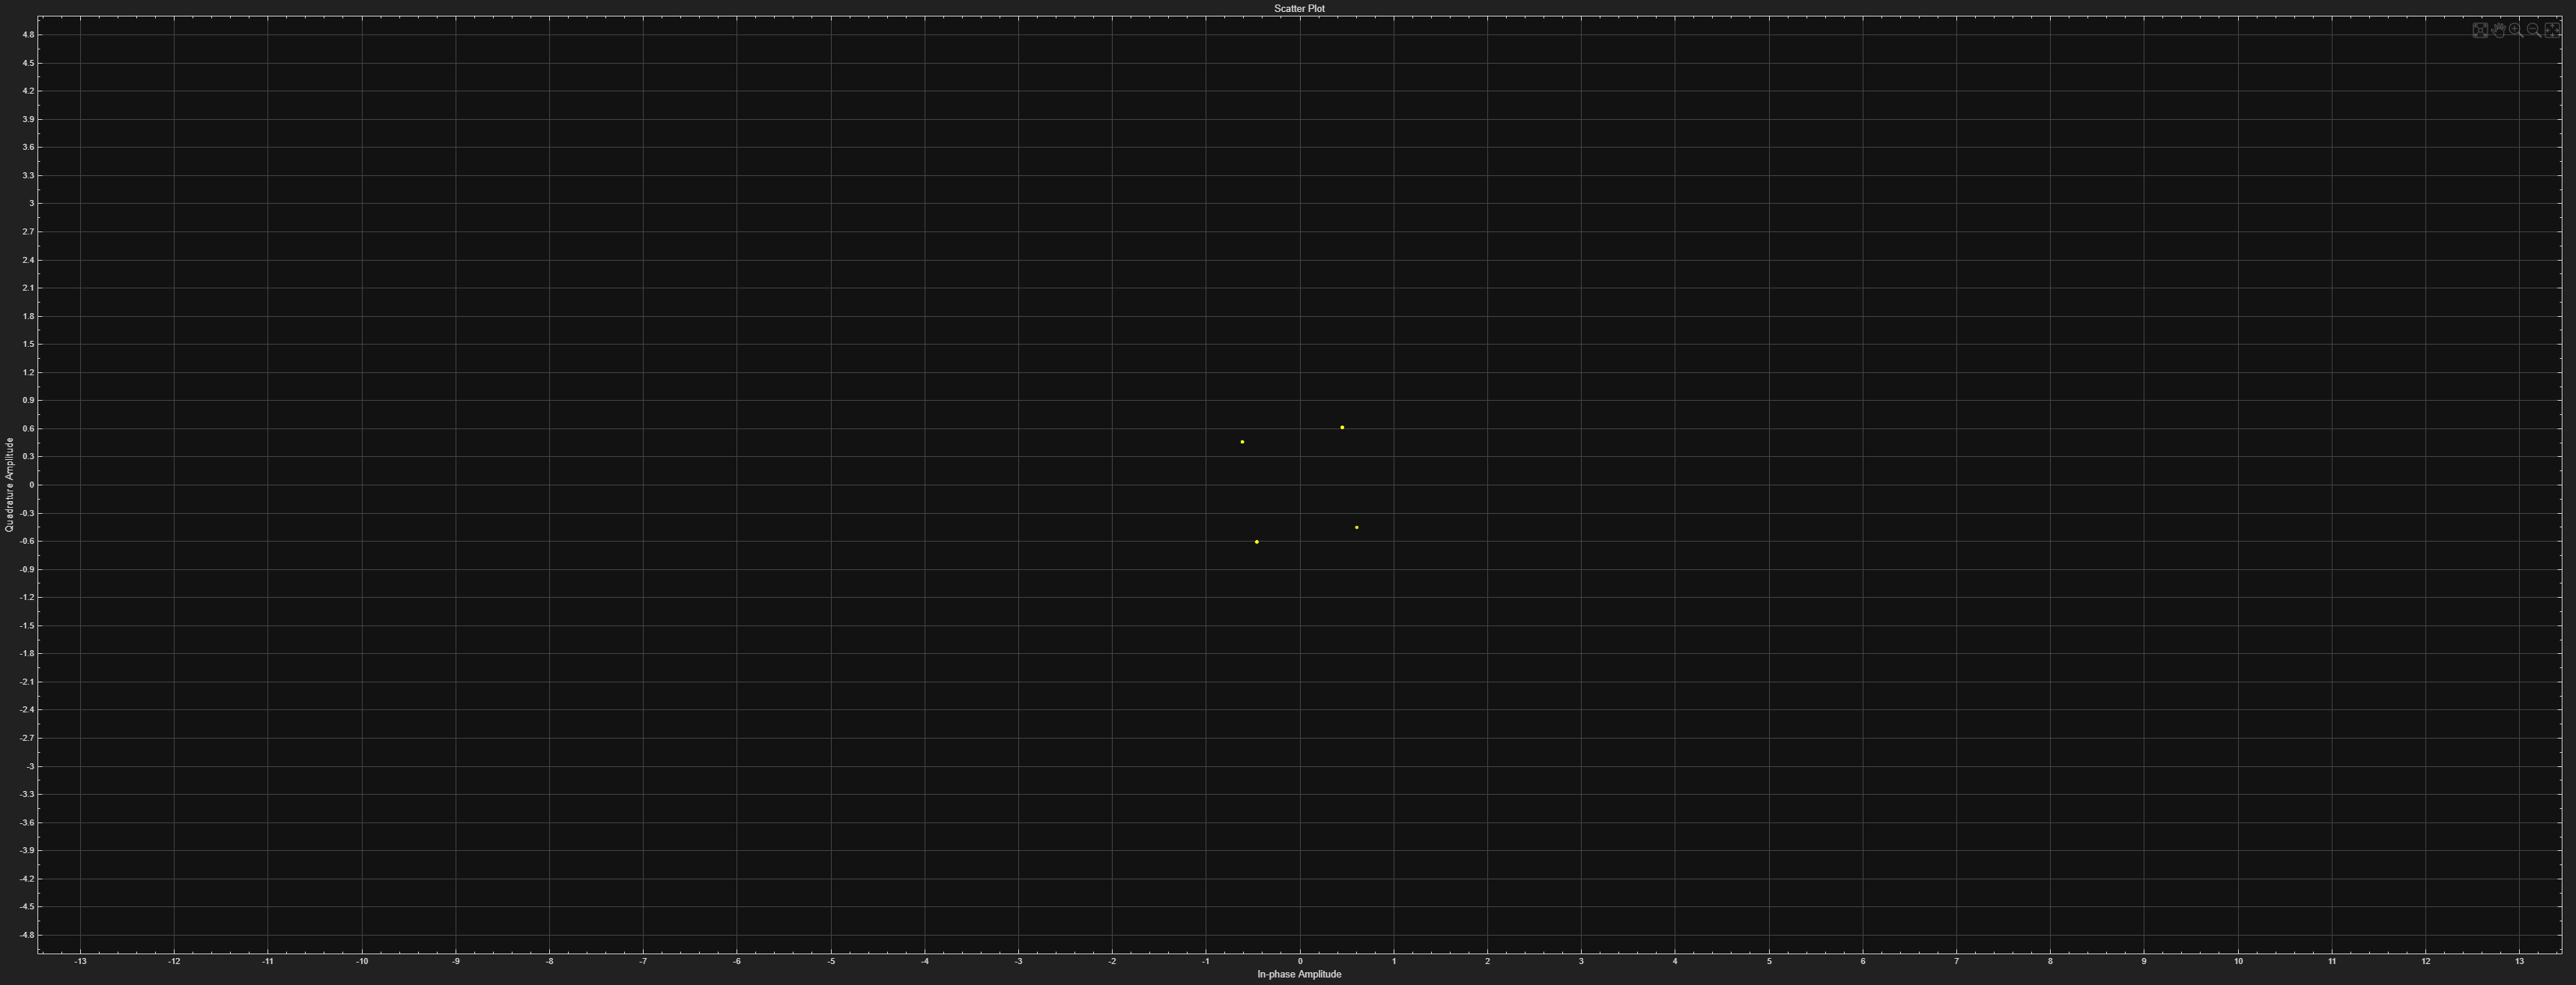
\includegraphics[width=\textwidth]{ric/ricconstpip2.png}
         \caption{$\frac\pi 2$ maximális fázistolású konstellációs diagram}
         \label{fig:ric_const2}
     \end{subfigure}
     \hfill
          \begin{subfigure}[b]{0.4\textwidth}
         \centering
         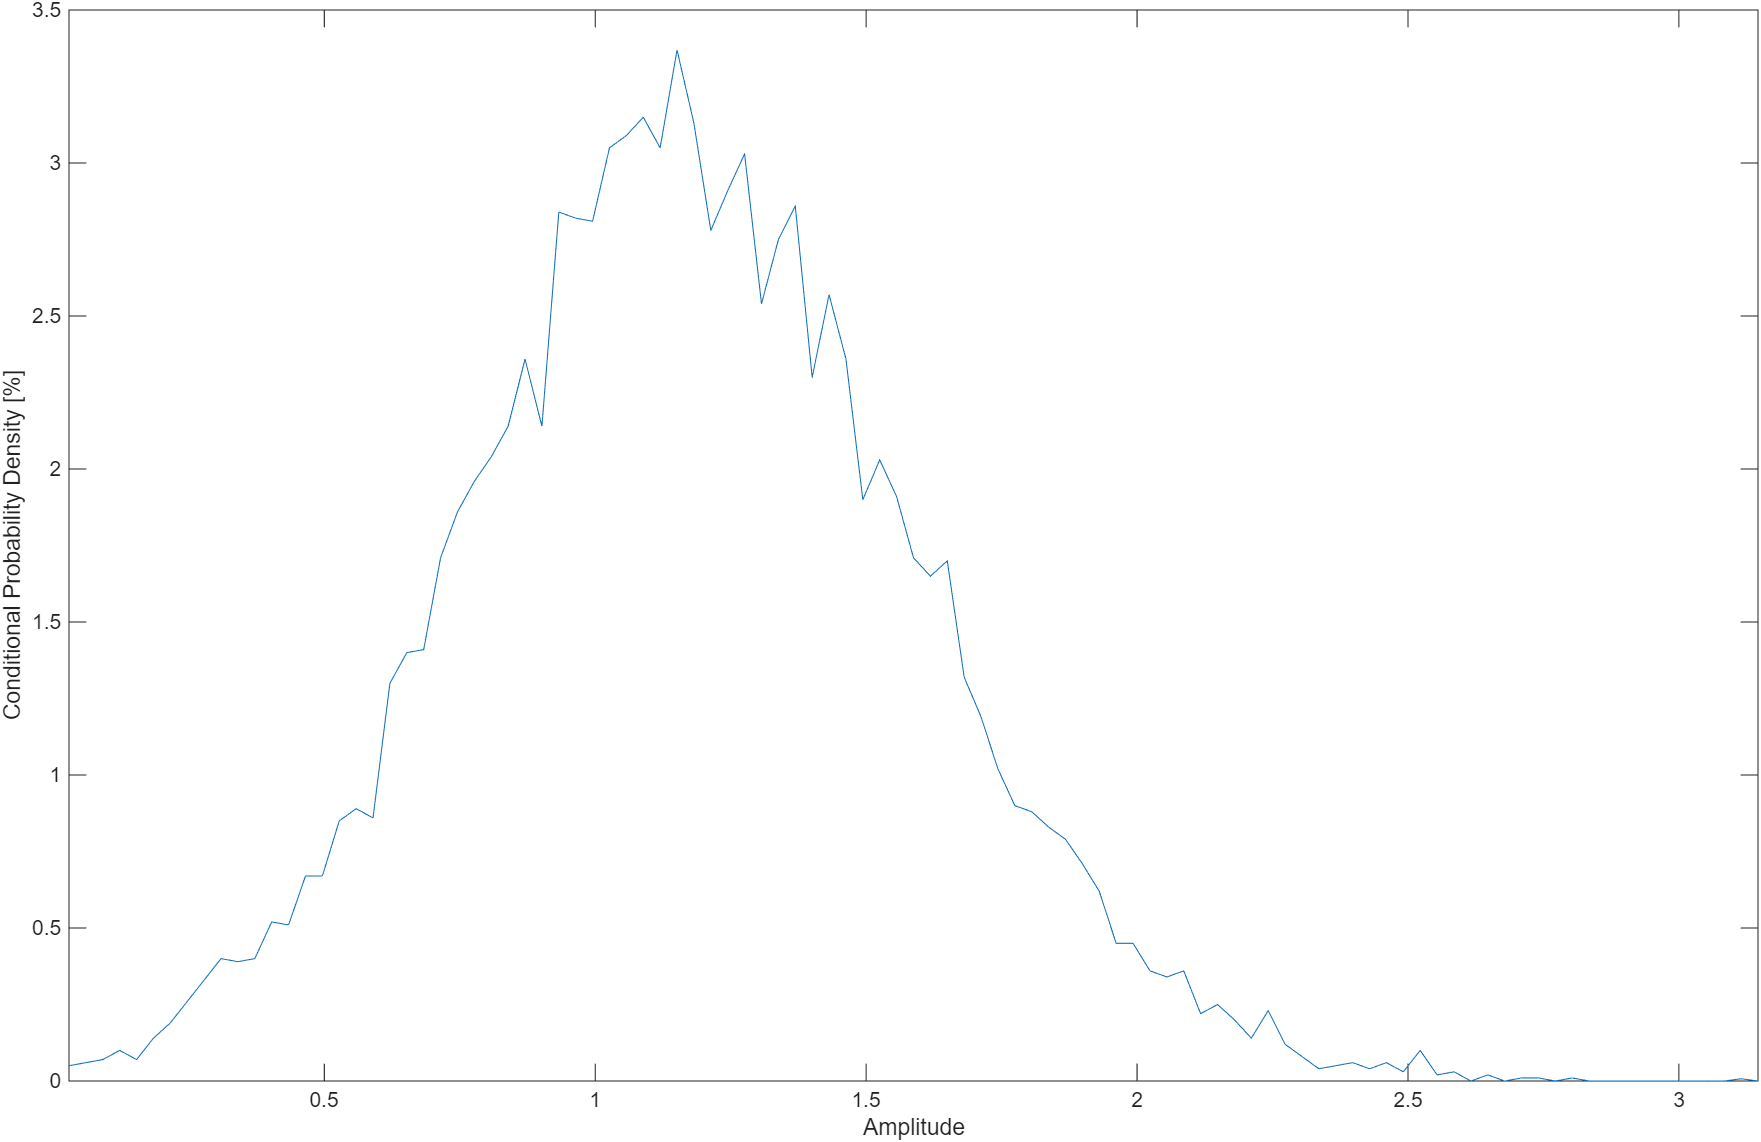
\includegraphics[width=\textwidth]{ric/ricdpip2.png}
         \caption{$\frac\pi 2$ maximális fázistolású eloszlás}
         \label{fig:ric_d2}
     \end{subfigure}
     \hfill
     \begin{subfigure}[b]{0.5\textwidth}
         \centering
         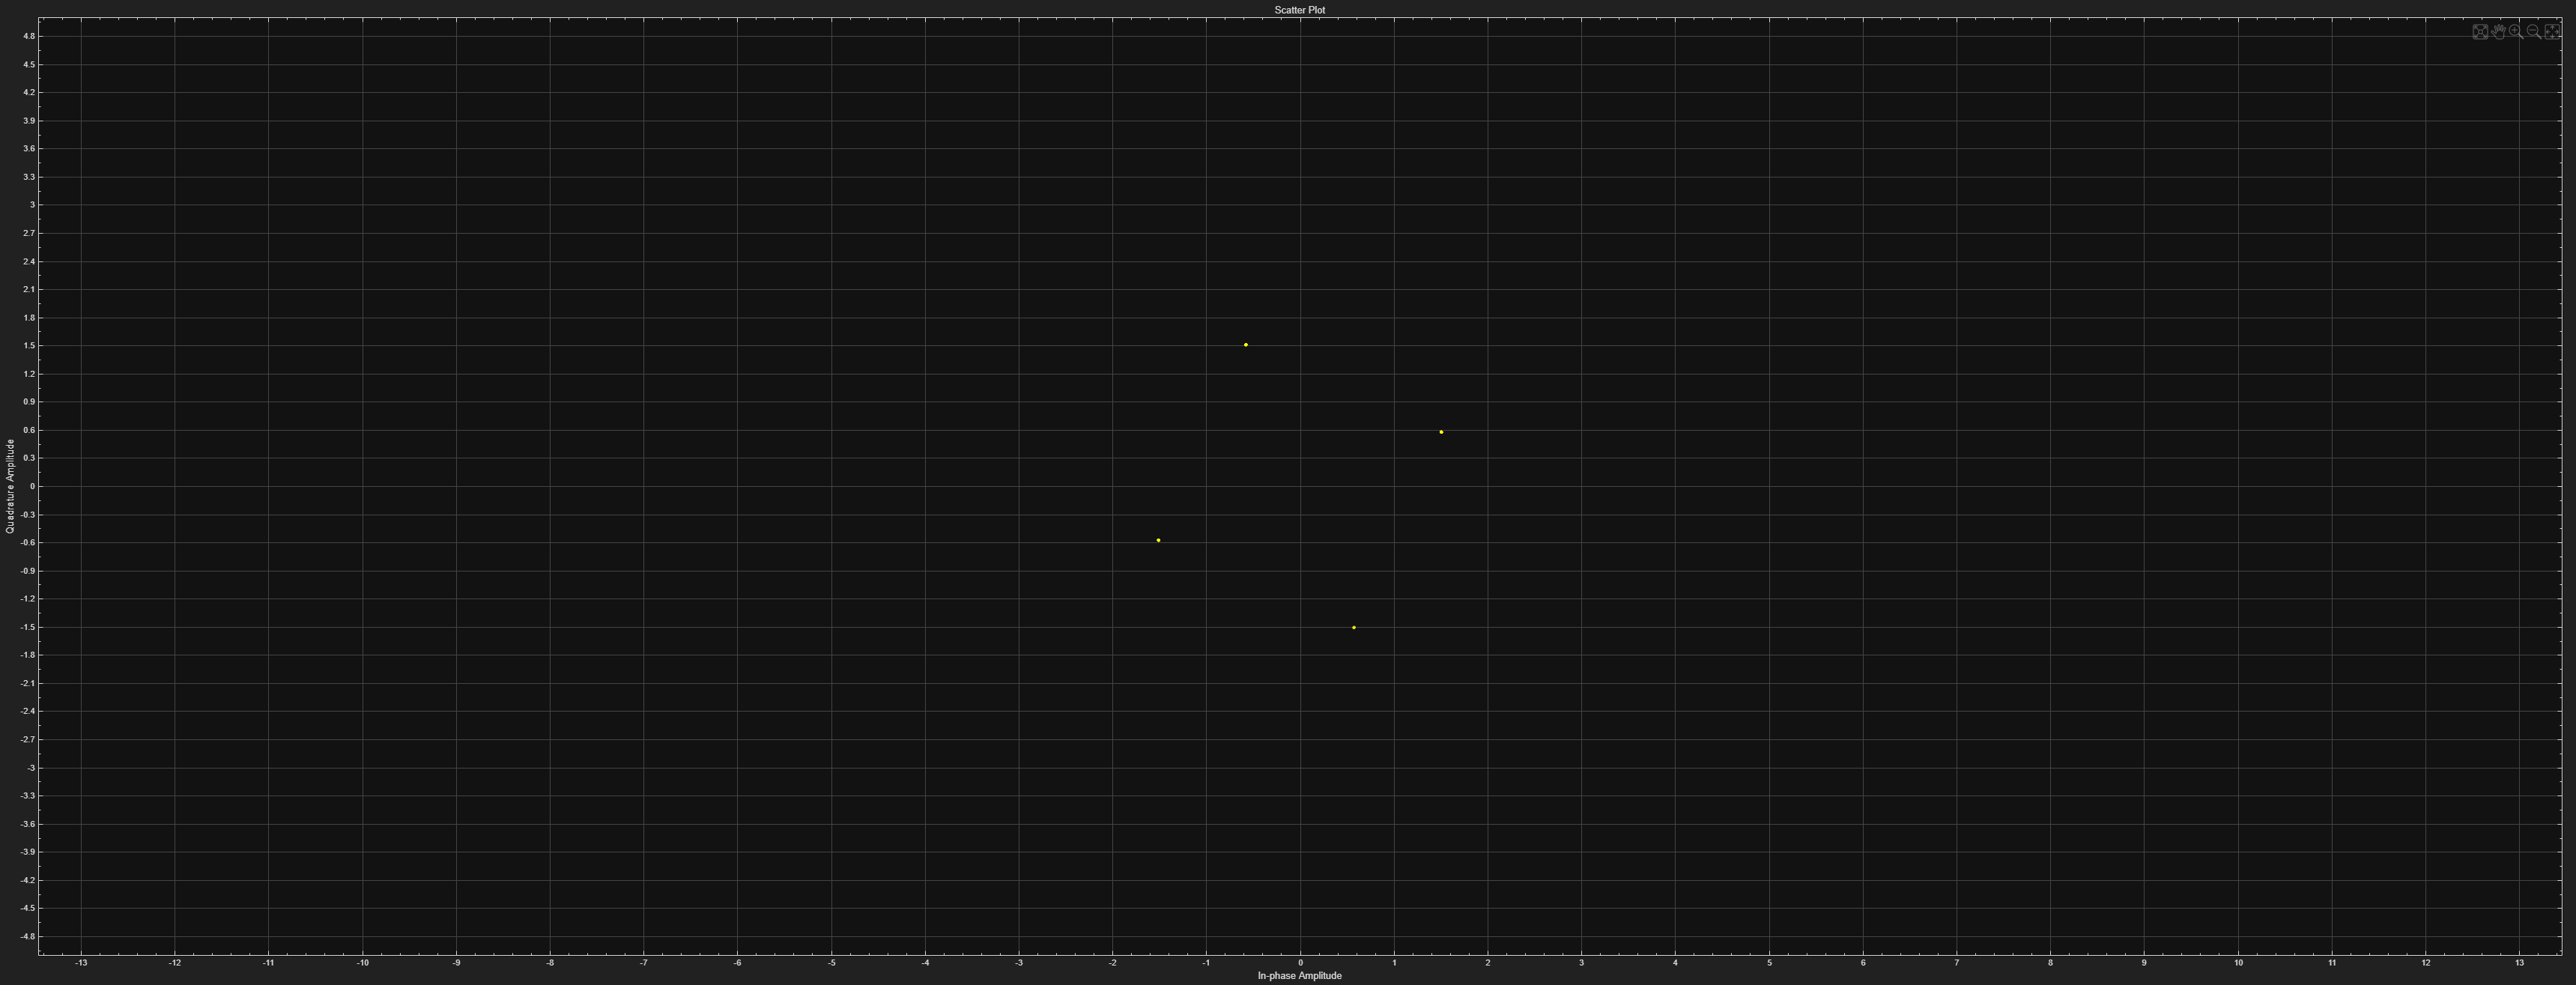
\includegraphics[width=\textwidth]{ric/ricconstpi.png}
         \caption{$\pi$ maximális fázistolású konstellációs diagram, 0,4-re növelt amplitúdó szórással}
         \label{fig:ric_const1}
     \end{subfigure}
     \hfill
     \begin{subfigure}[b]{0.4\textwidth}
         \centering
         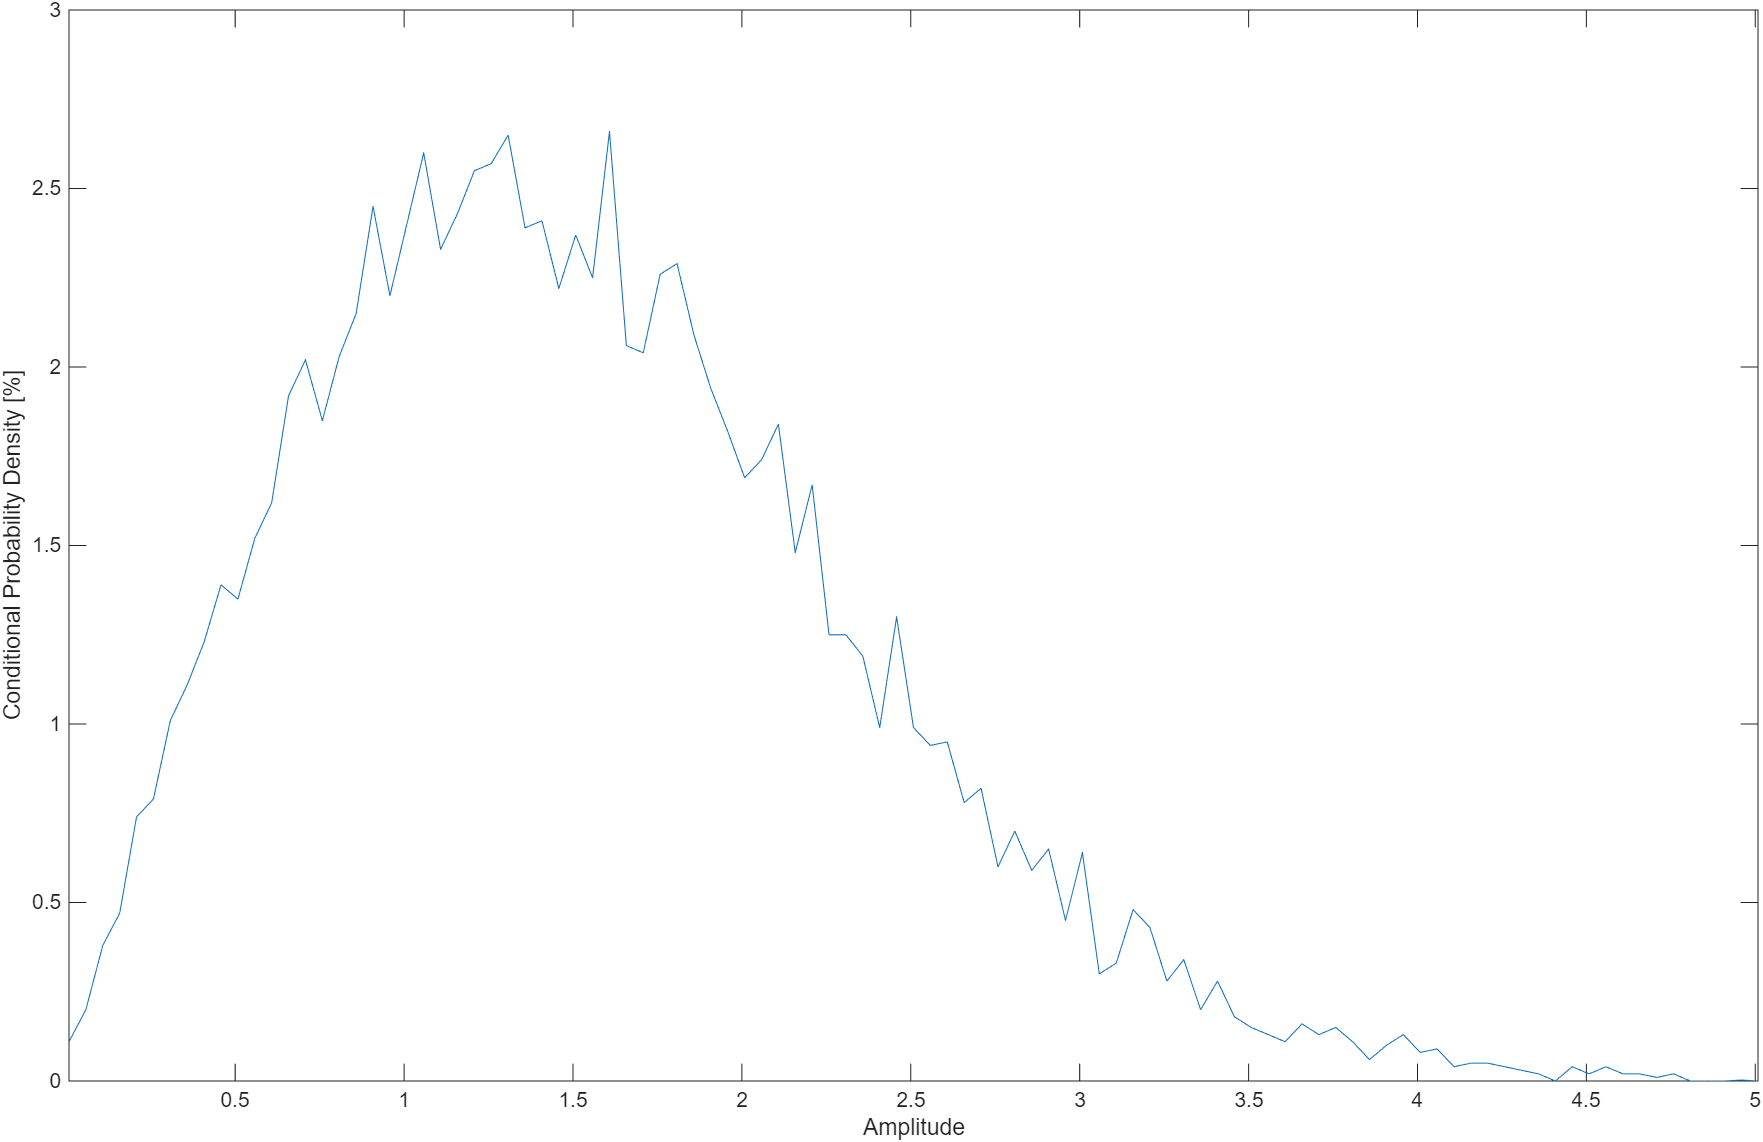
\includegraphics[width=\textwidth]{ric/ricdpi.png}
         \caption{$\pi$ maximális fázistolású eloszlás, 0,4-re növelt amplitúdó szórással}
         \label{fig:ric_d1}
     \end{subfigure}
        \caption{A Rice Csatorna szimuláció konstellációs diagramjai és eloszlásfüggvényei különböző maximális fázistolások és amplitúdó szórások mellett}
        \label{fig:ric_res}
\end{figure}

\begin{table}[h]
    \centering
    \begin{tabular}{|c|c|c|}\hline
    Paraméterek & $\phi_\text{max}=\pi/2,\ \sigma_A=0.05$ & $\phi_\text{max}=\pi,\ \sigma_A=0.4$\\\hline
    Hibaarány [\%] & 7,289 & 42,48 \\\hline
    \end{tabular}
    \caption{A Rice Modell különböző maximális fázistolásokhoz és amplitúdó szórásokhoz tartozó
hibaarányai}
    \label{tab:ricErr}
\end{table}
A mérési eredmények alapján megállapítható, hogy a Rice-csatorna a közvetlen rálátású (LOS) komponens jelenléte miatt megbízhatóbb átvitelt biztosít, mint a  Rayleigh-modell.Az első vizsgált esetben ($\phi_{\text{max}}=\frac\pi2, \sigma_A=0.05$) kapott 7,29\%-os hibaarányt kaptunk, míg a Rayleigh modell esetén ekkor már 50\% feletti volt a hiba. Ez a hibaarány hibajavító kódolással még kezelhető. A második esetben, ahol a fázistolást $\pi$-re, az amplitúdószórást pedig $\sigma_A=0.4$-re növeltük, a hibaarány 42,48\%-ra emelkedett. Ekkor már a csatorna erősen zavaros, érdemi jelátvitel nehezen/szinte egyáltalán nem valósítható meg. Jól látható \aref{fig:ray_ric}.~ábráról és a szimulált eredmények alapján is, hogy a két esetben eltér az amplitúdó időbeli eloszlásfüggvénye, mivel  $\sigma_A$ értékét változtattuk a későbbi mérési feladat során.
\section{Log-normál csatornamodell}
\subsection{Elméleti háttér}
A következő modell a Log-normál csatornamodell.
Log-normál csatornamodell esetén az adó- és vevőantenna között különböző elnyelő térfogatok találhatók, az átviteli út teljes csillapítása ezen térfogatok különböző $a_i$ csillapításainak szorzataként adódik. Logaritmikus skálán a teljes csillapítás az $A_i$ részcsillapítások összege: \[\sum \ln a_i=\sum A_i.\]
% <esetleg néhány fiszemfaszomábra a segéletből>

A log-normál csatornamodell kiválóan alkalmas az olyan környezeti hatások leírására, mint például az eső okozta jelcsillapítás. Ez esetben az adó és a vevő közötti összeköttetés mentén különböző kiterjedésű és sűrűségű elnyelő térfogatok (esőzónák) helyezkednek el.

\subsection{Mérési feladatok, mérés menete}
A log-normál modell vizsgálatát az előzőekben is használt eljárással hajtottuk végre. Itt a vizsgált paraméter a különböző csillapítású zónákat szimuláló alrendszerek csillapításának felső határértéke.\footnote{\label{ftn:minmax}A Simulink modellben a csillapítás növeléséhez a jelhez adott véletlen érték minimumát állítjuk egyre kisebbre.}
\begin{figure}[h]
    \centering
    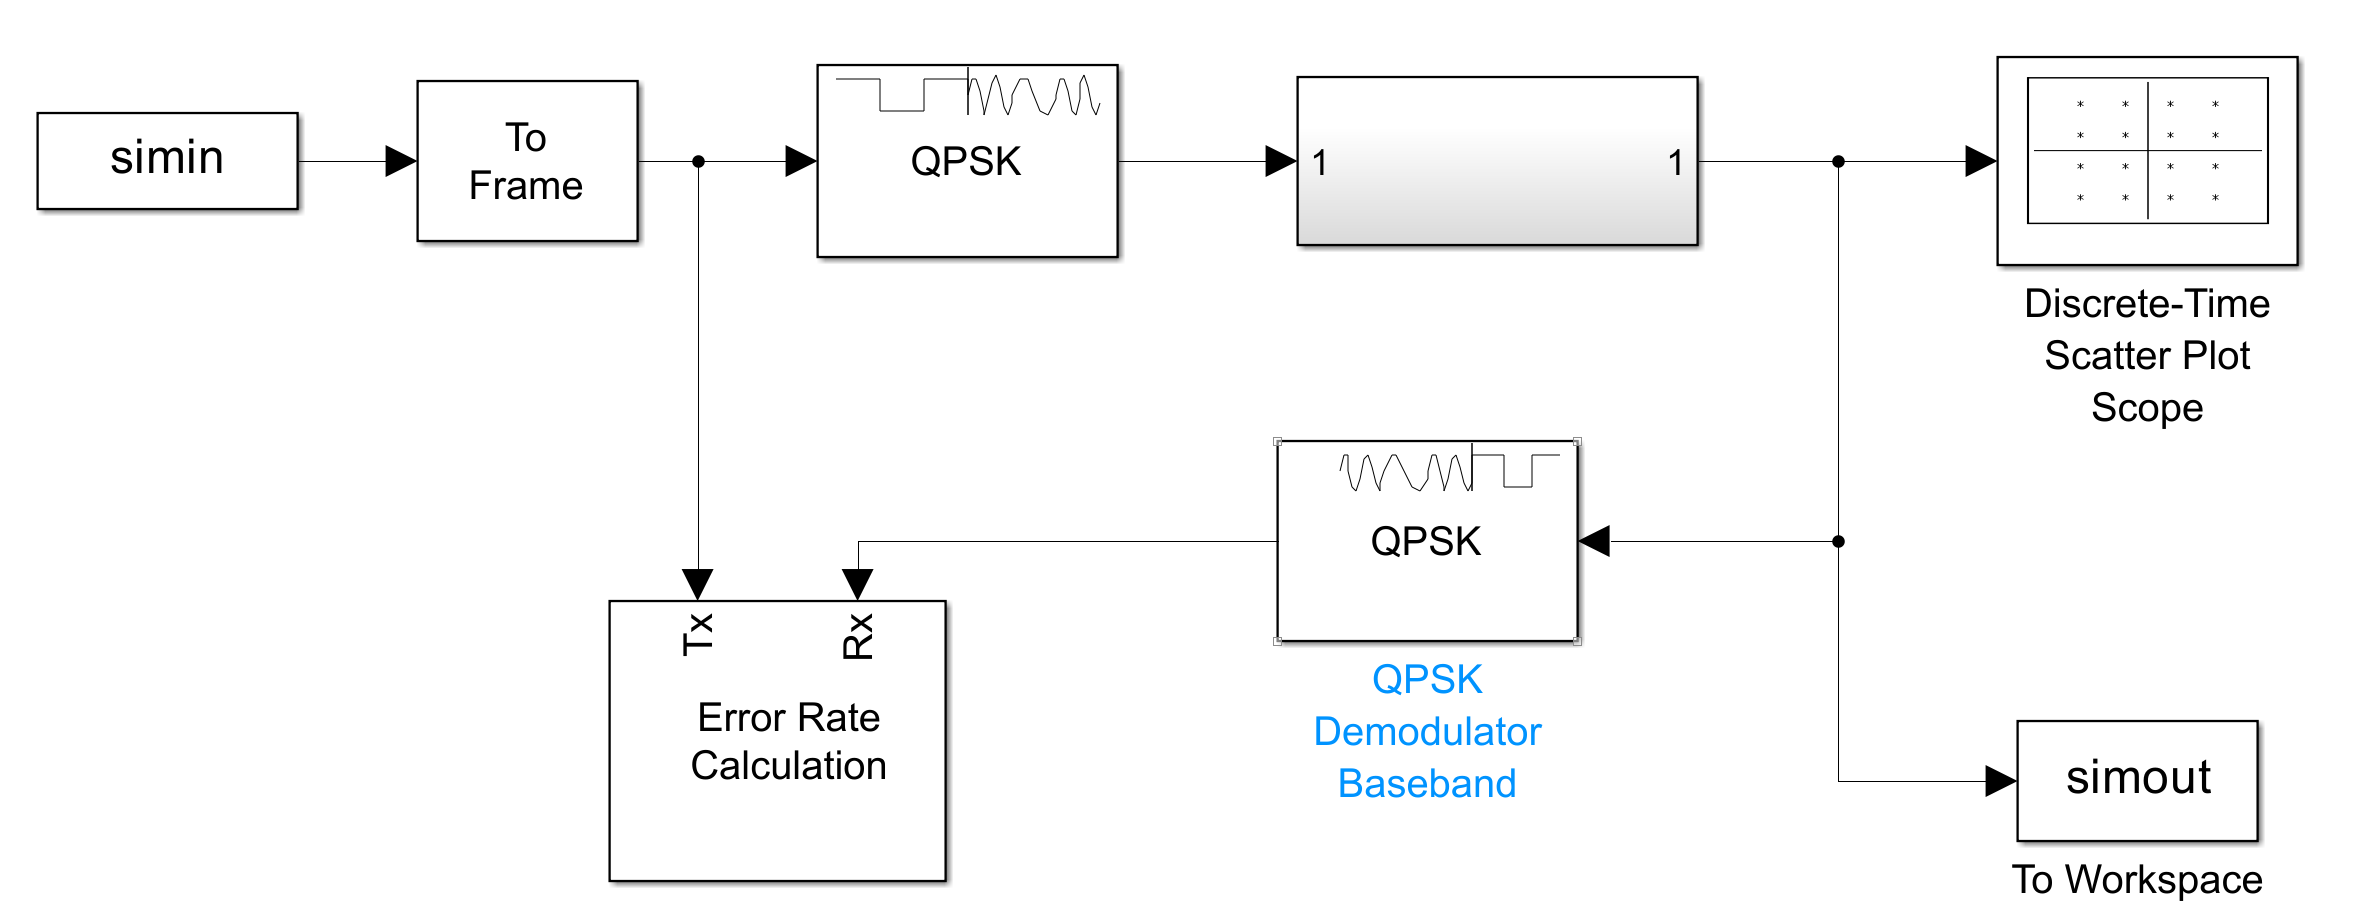
\includegraphics[width=0.6\linewidth]{lgn/lgn_mod.png}
    \caption{A használt Log-normál csatornamodell}
    \label{fig:lgnmod}
\end{figure}

\begin{figure}[htbp]
     \centering
     \begin{subfigure}[b]{0.7\textwidth}
         \centering
         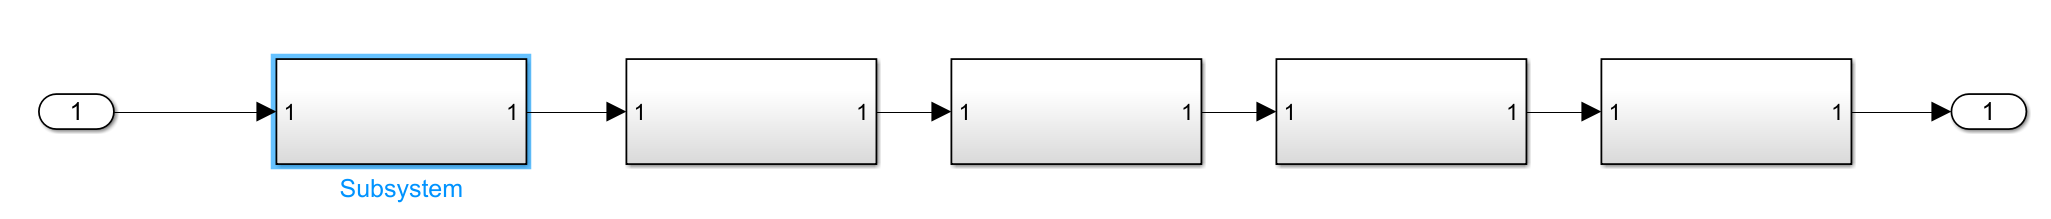
\includegraphics[width=\textwidth]{lgn/lgn_set1.png}
         \caption{Több csillapító térfogat szimulációja}
         \label{fig:lgn_set_multattenuation}
     \end{subfigure}
     \hfill
          \begin{subfigure}[b]{0.6\textwidth}
         \centering
         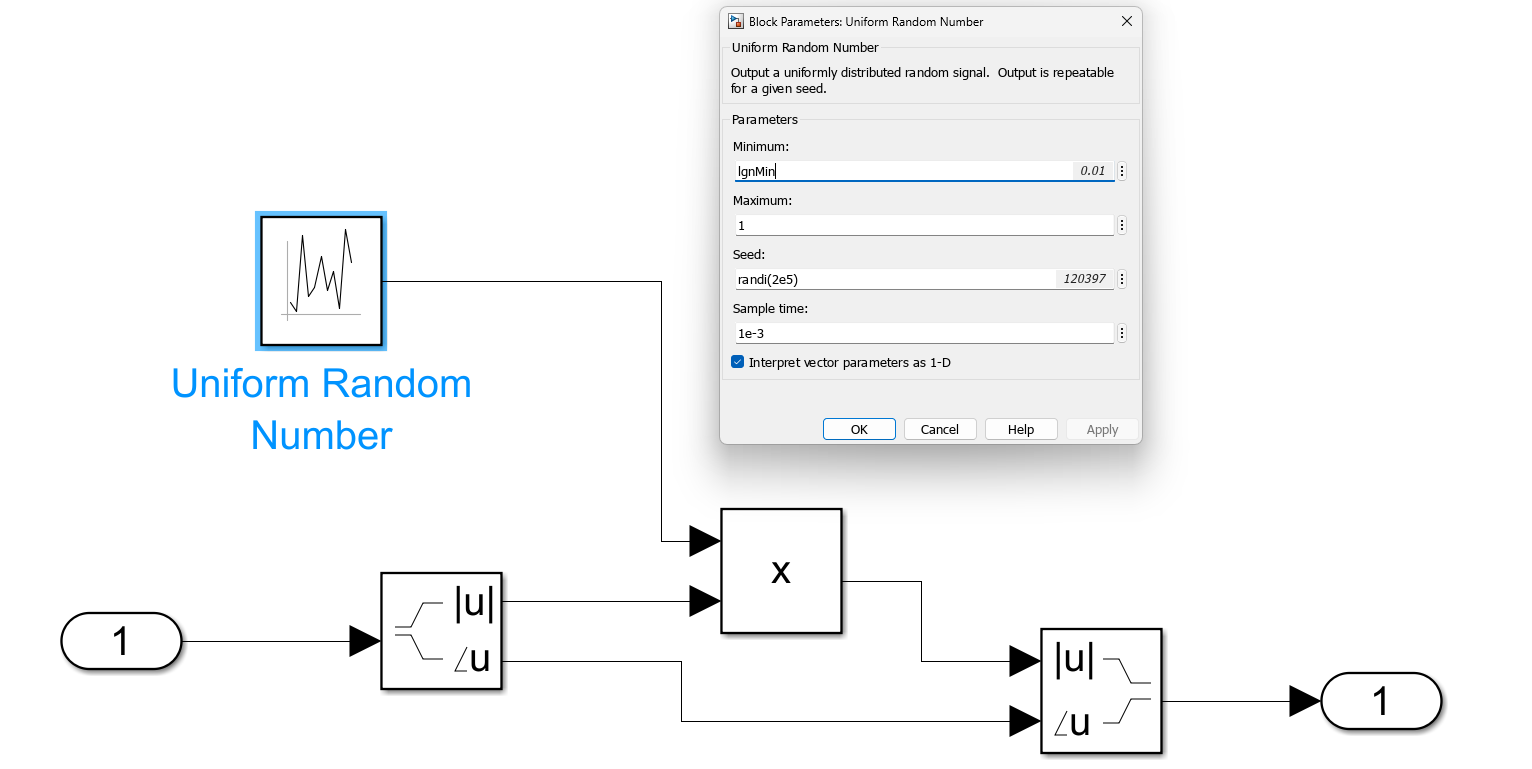
\includegraphics[width=\textwidth]{lgn/lgn_set2.png}
         \caption{A maximális csillapítást az \texttt{lgnMin}\footnotemark{} változó befolyásolja}
         \label{fig:lgn_set_noise}
     \end{subfigure}
        \caption{A szimulációs modell belső felépítése}
        \label{fig:ray_set}
\end{figure}
\footnotetext{{Lásd: \ref{ftn:minmax}.~lábjegyzet}}
\subsection{Kapott eredmények, értékelés}

\begin{figure}[ht]
     \centering
     \begin{subfigure}[b]{0.5\textwidth}
         \centering
         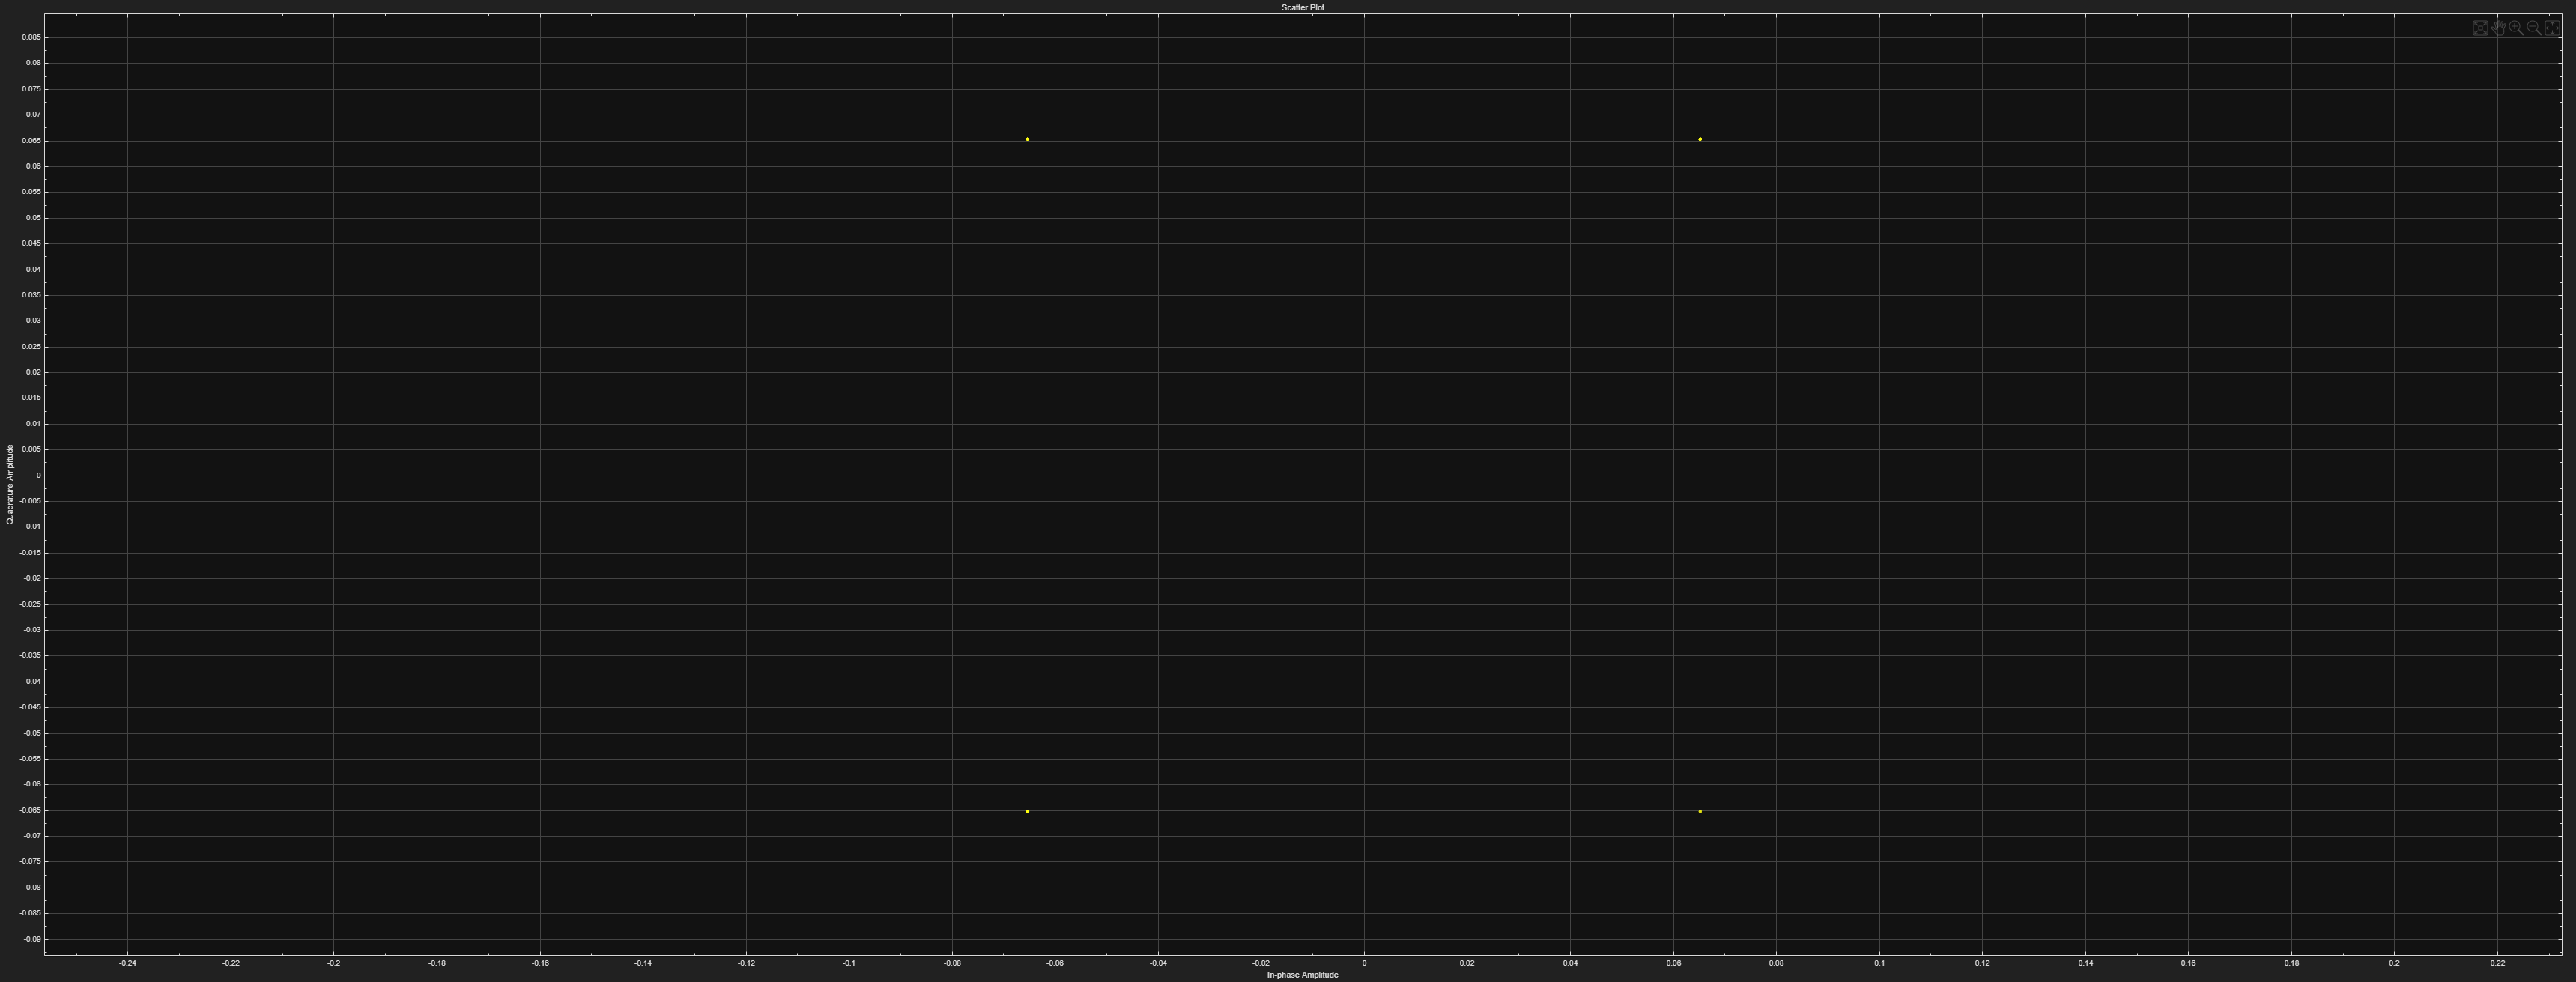
\includegraphics[width=\textwidth]{lgn/lgnconst001.png}
         \caption{0,01 maximális csillapítású konstellációs diagram}
         \label{fig:ric_const2}
     \end{subfigure}
     \hfill
          \begin{subfigure}[b]{0.4\textwidth}
         \centering
         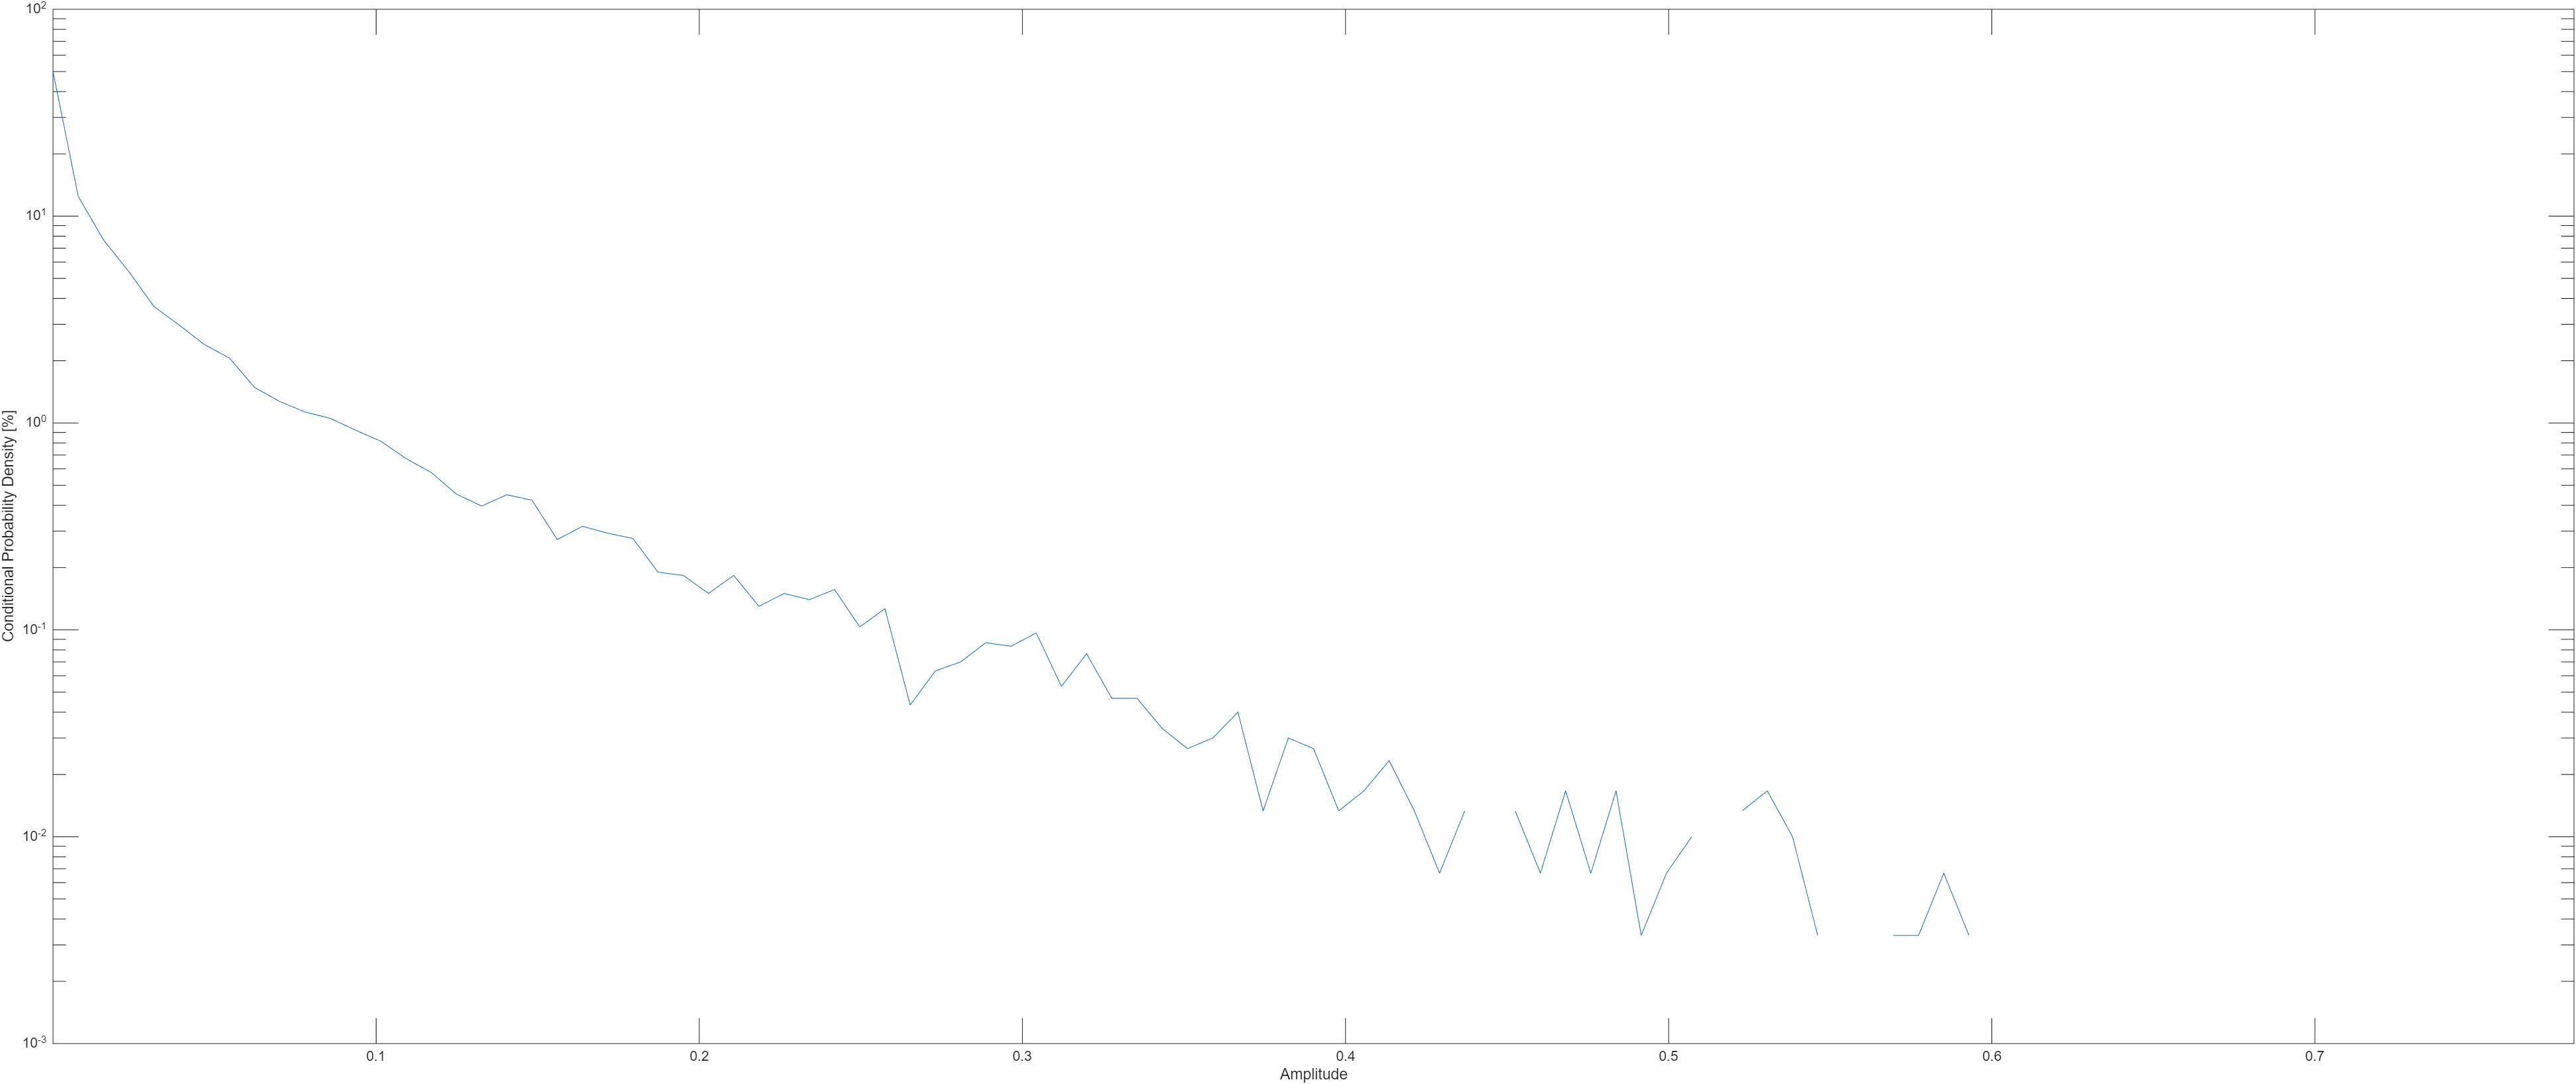
\includegraphics[width=\textwidth]{lgn/lgnd001.png}
         \caption{0,01 maximális csillapítású eloszlás}
         \label{fig:ric_d2}
     \end{subfigure}
     \hfill
     \begin{subfigure}[b]{0.5\textwidth}
         \centering
         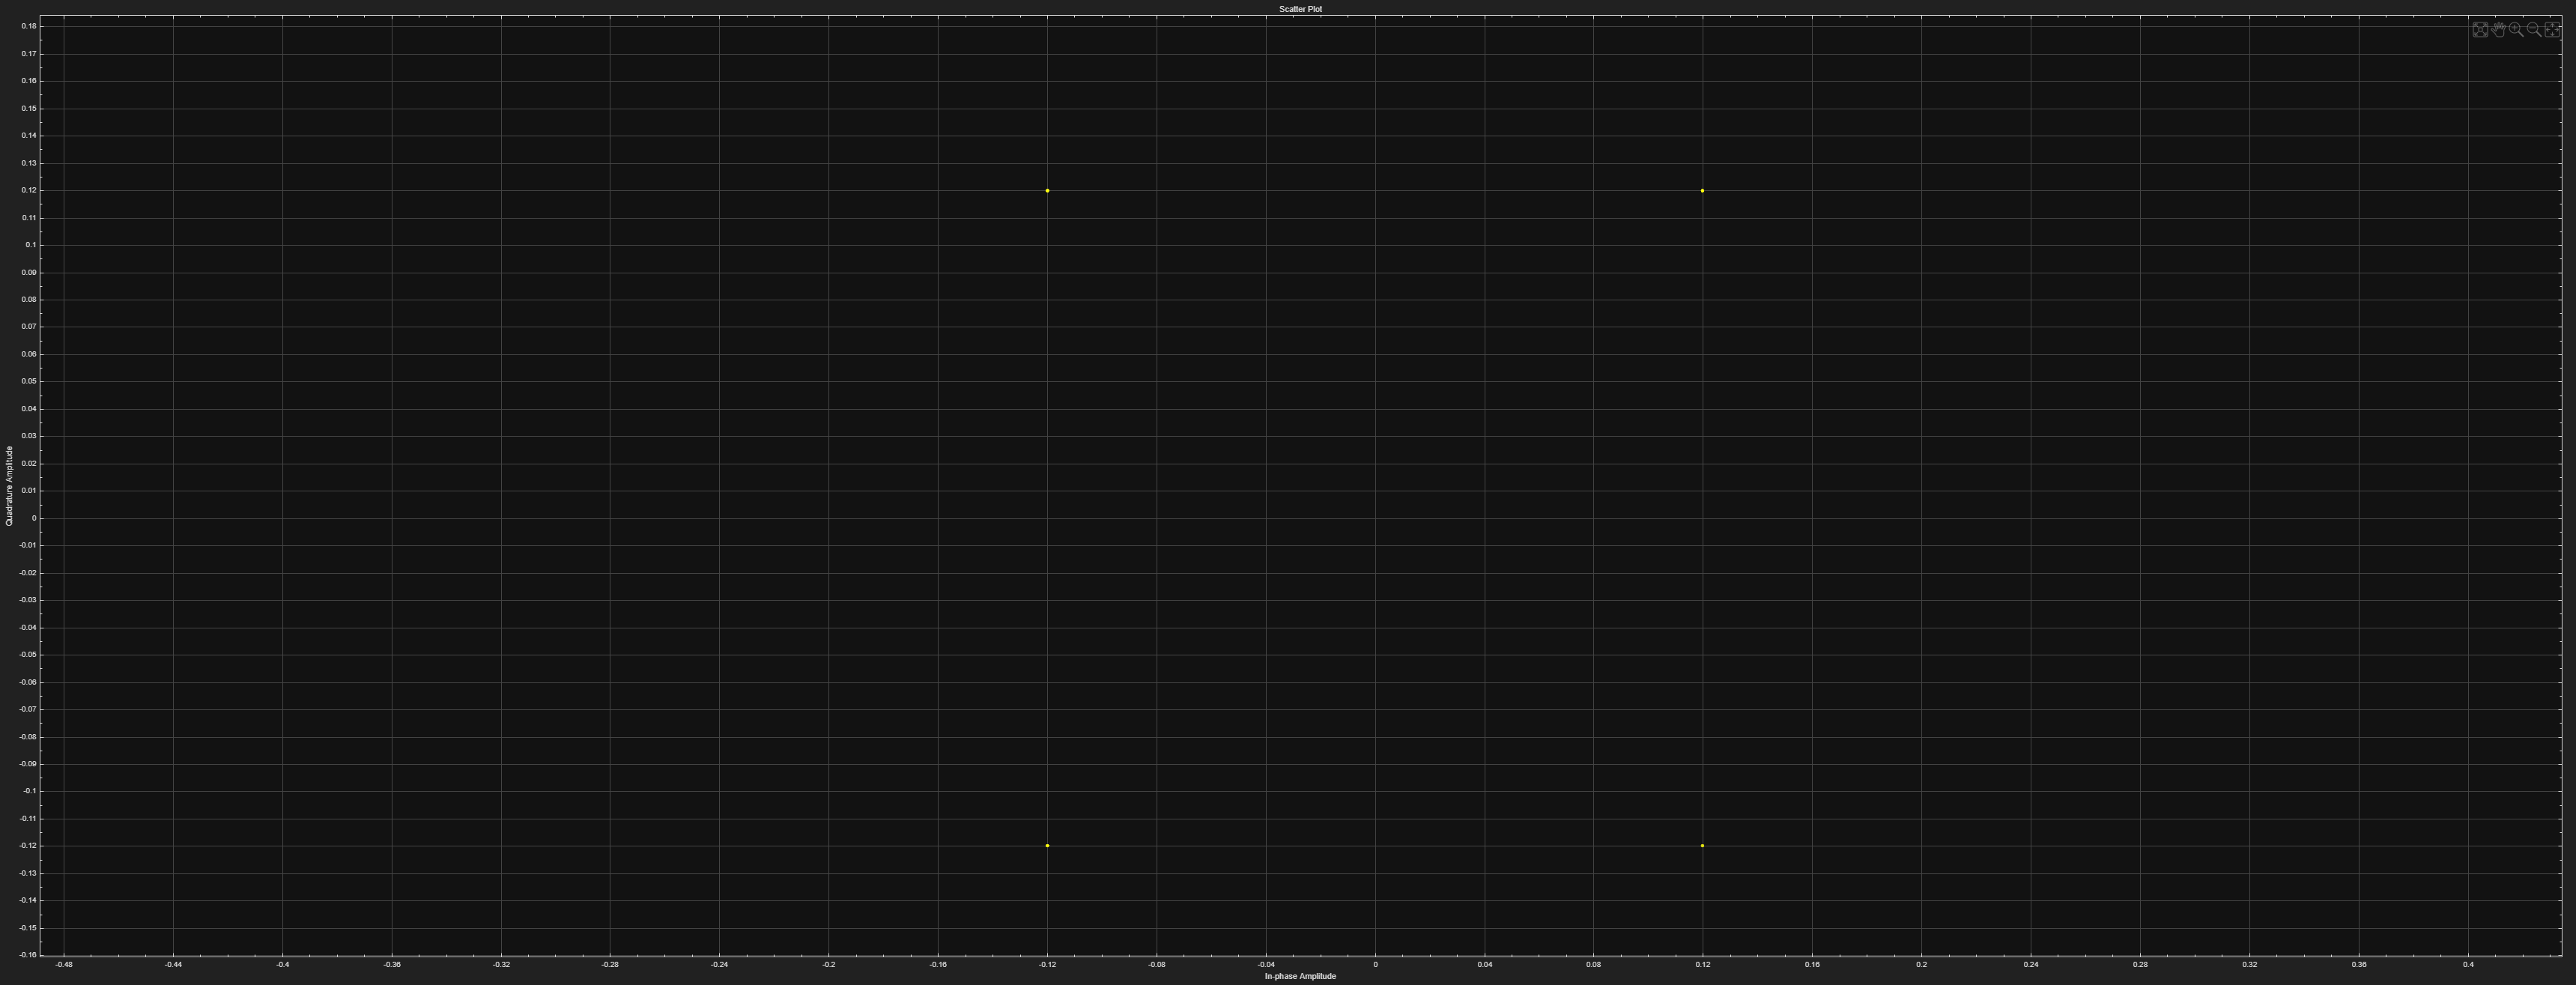
\includegraphics[width=\textwidth]{lgn/lgnconst01.png}
         \caption{0,1 maximális csillapítású konstellációs diagram}
         \label{fig:ric_const1}
     \end{subfigure}
     \hfill
     \begin{subfigure}[b]{0.4\textwidth}
         \centering
         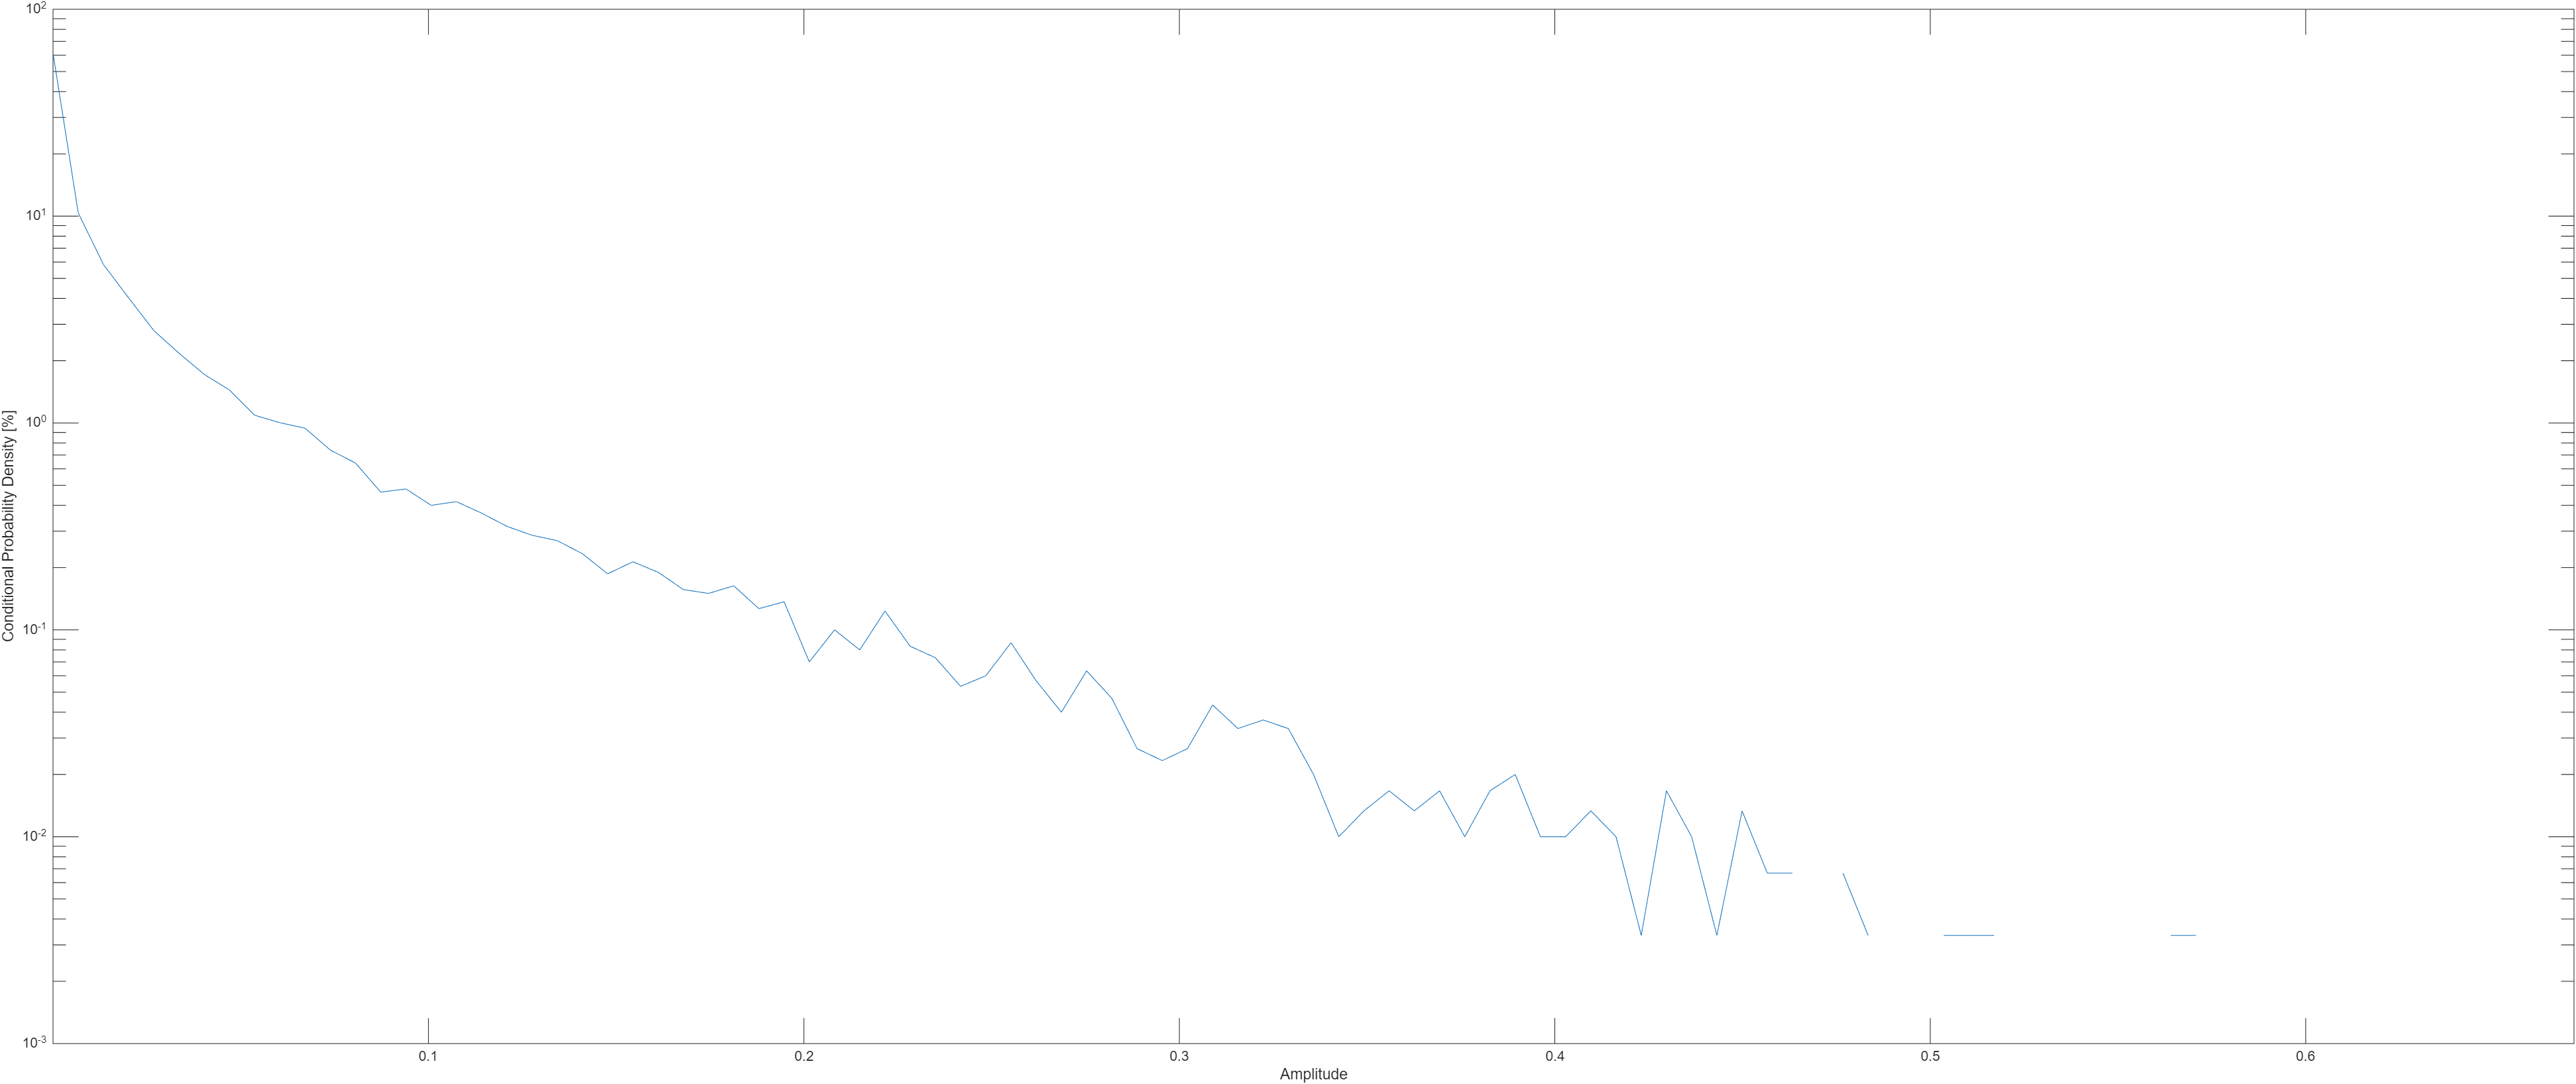
\includegraphics[width=\textwidth]{lgn/lgnd01.png}
         \caption{0,1 maximális csillapítású eloszlás}
         \label{fig:ric_d1}
     \end{subfigure}
        \caption{A Log-normál Csatorna szimuláció konstellációs diagramjai és eloszlásfüggvényei különböző maximális csillapítások mellett}
        \label{fig:ric_res}
\end{figure}

\begin{table}[h]
    \centering
    \begin{tabular}{|c|c|c|}\hline
    $a_\text{max}$ & 0,01 & 0,1 \\\hline
    Hibaarány [\%] & 4,7 & 31,7 \\\hline
    \end{tabular}
    \caption{A Log-normál Modell különböző maximális csillapítás értékekhez tartozó hibaarányai}
    \label{tab:lgnErr}
\end{table}

\section{Időjárási jelenségeket leíró csatornamodellek}
\subsection{Elméleti háttér}
\label{sec:raintheory}
A rádióhullámok terjedését jelentősen befolyásolják a környezeti tényezők, különösen az eső, a köd és a szél, amelyek extra csillapítást okoznak a csatornában. Ez a hatás főként a 10 GHz feletti frekvenciatartományban válik kritikussá, mivel itt a hullámhossz már összemérhetővé válik a csapadékcseppek fizikai méretével. A pontos terjedési modellezéshez a frekvencia mellett a hullámhosszt és a polarizációt is figyelembe kell vennünk, hiszen ezek mind hatással vannak az időjárás okozta fading nagyságára.

A földi mérések során a modellezéshez olyan adatokat rögzítünk, mint a hőmérséklet, a páratartalom, az $R$ esőintenzitás, valamint a szél sebessége és iránya. Ezen felül fontos rögzített adat még egy rádiós összeköttetésnél a vett jel teljesítménye, hiszen ennek a változásából is lehet időjárási körülményekre következtetni.

Statisztikai szempontból kiemelt jelentőségű a komplemens esőintenzitás függvény, amely megadja annak valószínűségét, hogy az eső intenzitása egy adott pontban meghalad-e egy kritikus $R_i$ értéket: $$F(R_i) = P(R > R_i).$$

A várható csillapítás számszerűsítésére az ITU-R esőcsillapítási modellt, illetve a félempirikus Moupfouma-modellt alkalmazzuk. Mindkét eljárás közös alapokra épül: a számításhoz szükséges bemenő paraméterként a vivőfrekvenciát, a polarizációt, a konkrét szakaszhosszt, valamint a mérésekből származó, $R_{0.01}$ éves 0,01\%-os valószínűségű esőintenzitást használják fel.

\subsection{Mérési feladatok, mérés menete}

Ehhez a feladathoz egy mérési célokra felállított rádiós összeköttetés és azzal párhuzamosan, közös helyen üzemeltetett meteorológiai állomás egyhavi adatait kaptuk. Az adatsorok feldolgozásával szemléltetnünk kellett a meteorológiai jelenségek -- elsősorban az eső -- rádiós átvitelre gyakorolt hatását. A szemléltetés céljából:
\begin{enumerate}
    \item diagramon ábrázoltuk az egyes napokon mért esőintenzitás, vett teljesítmény és hőmérséklet értékeket,
    \item hisztogramot generáltunk a vett teljesítményekről és
    \item a hisztogram alapján empirikus eloszlásfüggvényt generáltunk, amit összevetettünk \aref{sec:raintheory}.~fejezetben taglalt modellekkel.
\end{enumerate}
\subsection{Kapott eredmények, értékelés}

\Aref{fig:rain_stats}.~ábra adataiból szembetűnő, hogy az esőintenzitás erősen korrelál a rádiós csillapítással, valamint hogy a magasabb intenzitású eső a hőmérséklet csökkenését is előidézi.

\begin{figure}[ht]
    \centering
    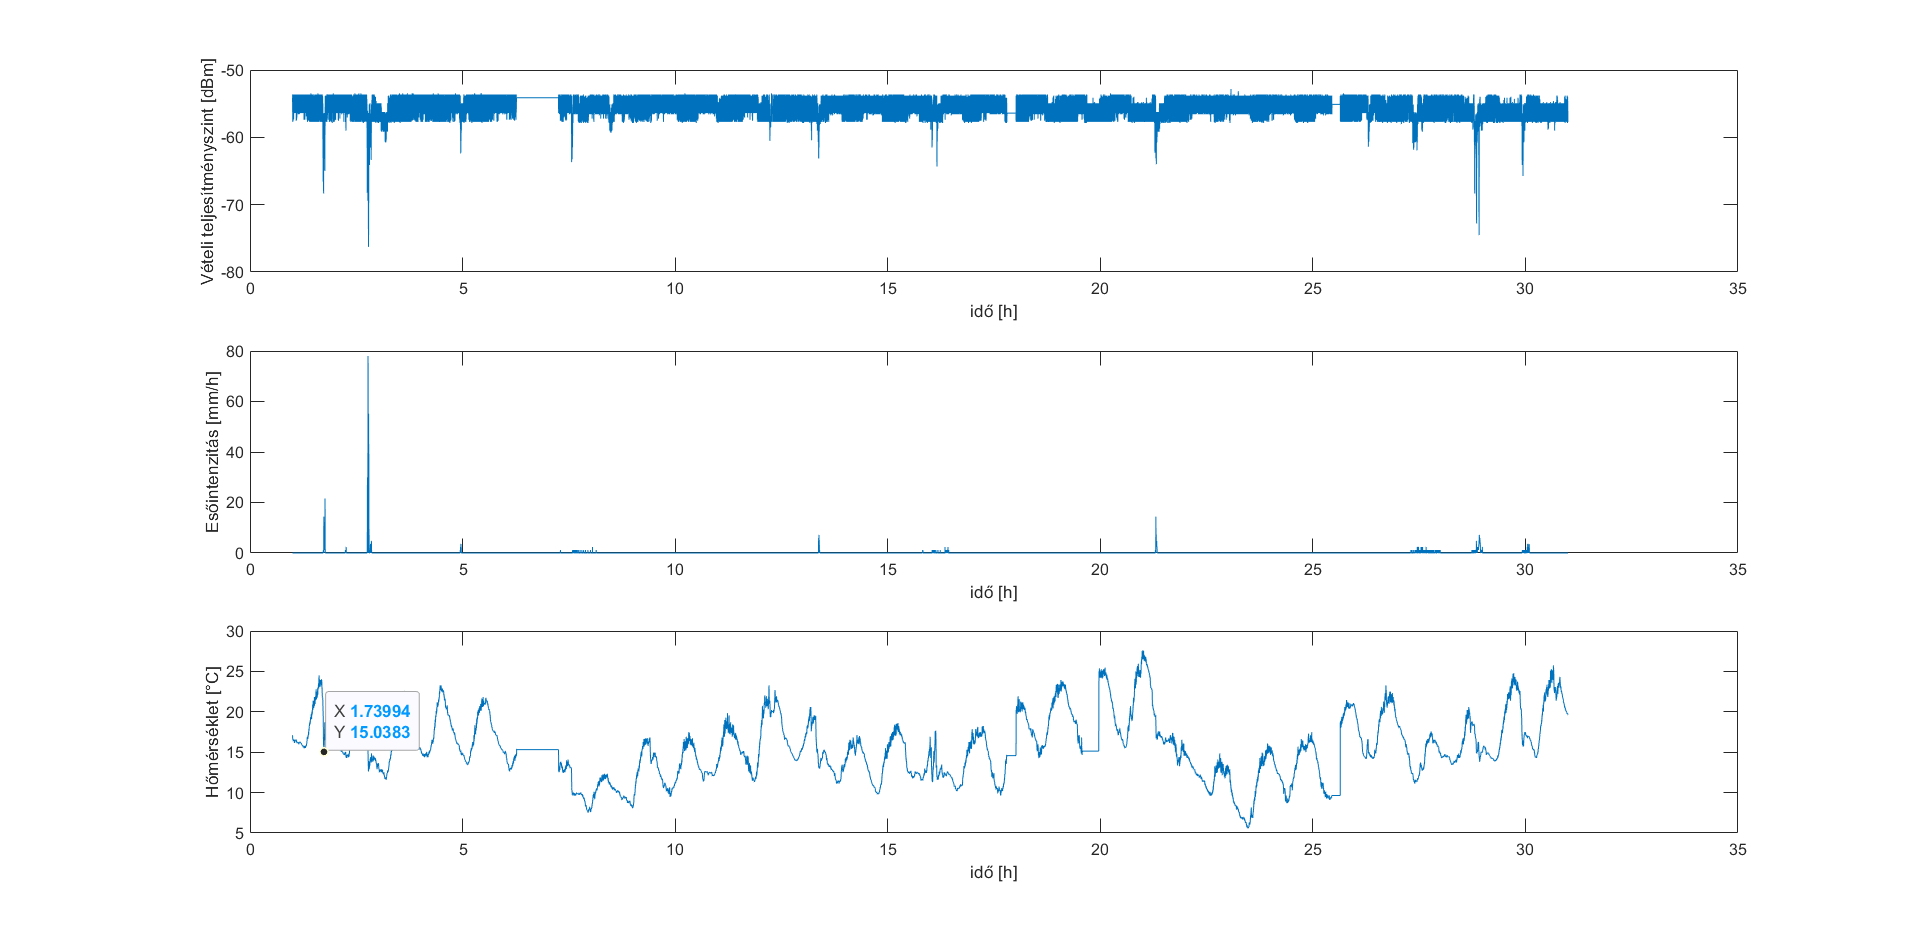
\includegraphics[width=0.75\linewidth]{rain/rain_stats.png}
    \caption{A mért adatok ábrázolása}
    \label{fig:rain_stats}
\end{figure}

\begin{figure}[h]
\centering
\begin{subfigure}{0.45\textwidth}
    \centering
    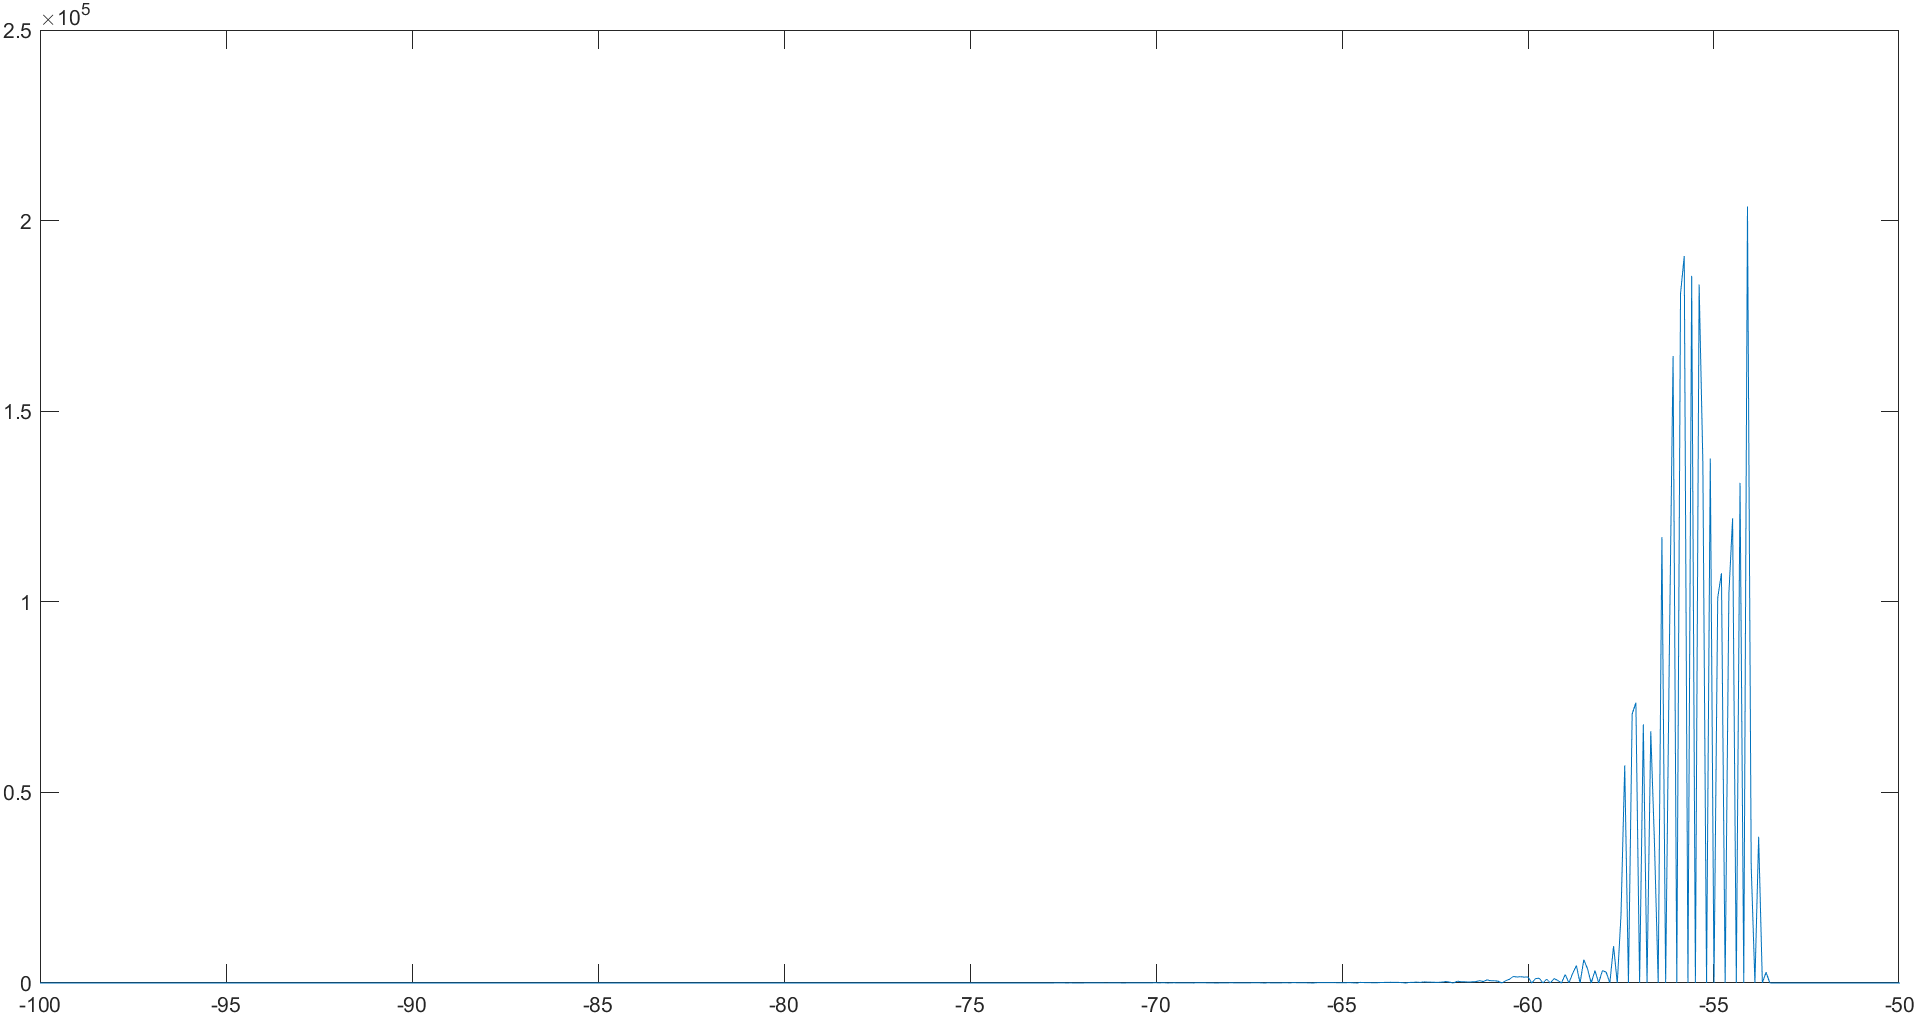
\includegraphics[width=\textwidth]{rain/rain_hist.png}
    \caption{A vett teljesítmények hisztogramja}
    \label{fig:rain_hist}  
\end{subfigure}
\hfill
\begin{subfigure}{0.45\textwidth}
    \centering
    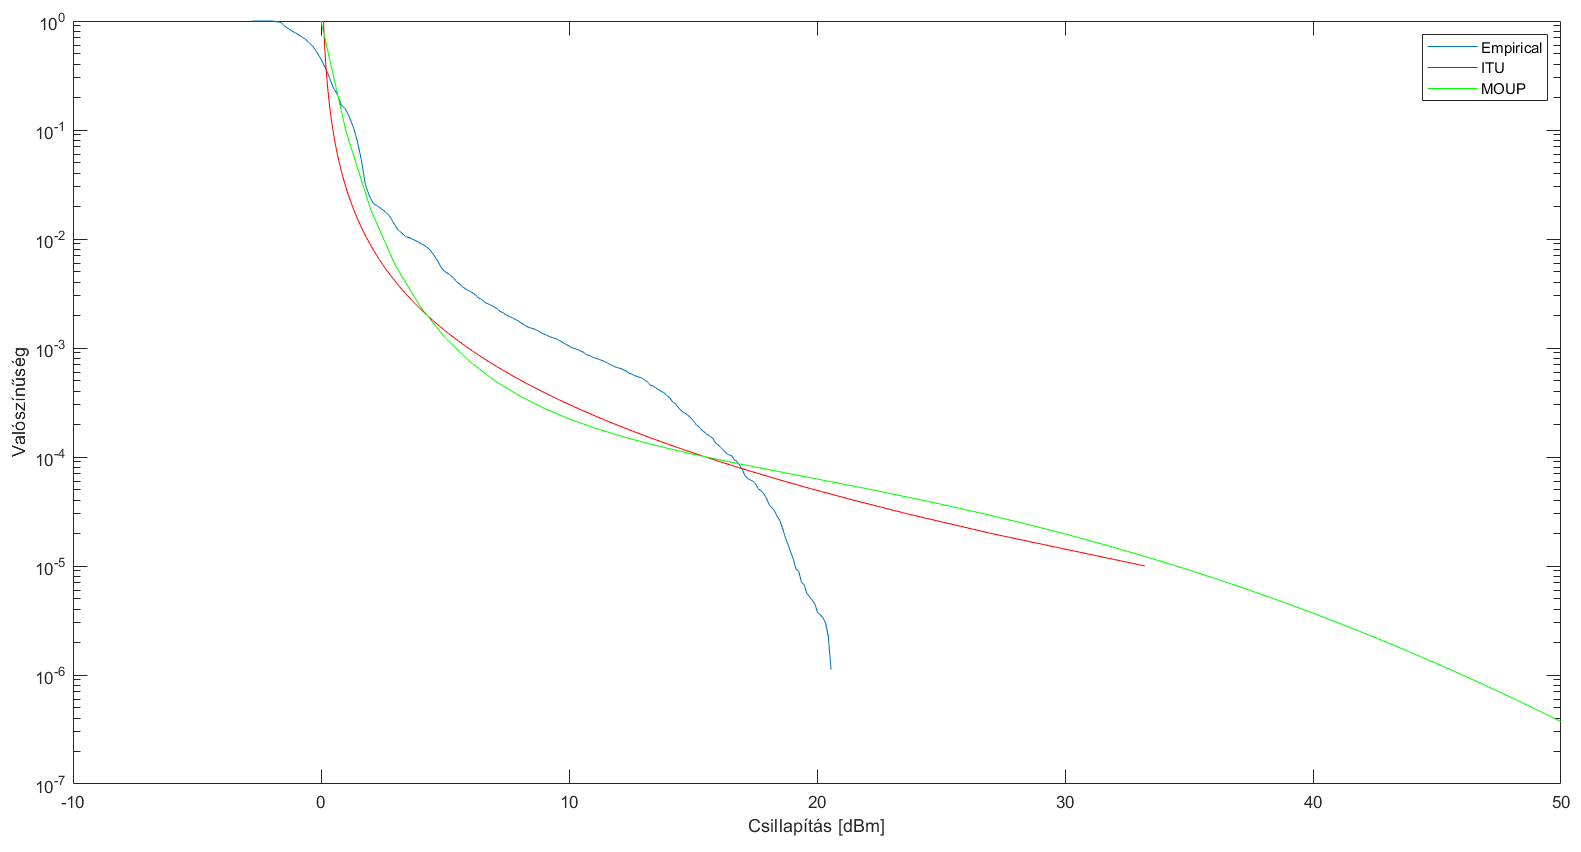
\includegraphics[width=\textwidth]{rain/rain_mods.png}
    \caption{A mért és elméleti modellek összehasonlítása}
    \label{fig:rain_mods}
\end{subfigure}
\caption{A teljesítmény hisztogramja és eloszlása}
\end{figure}

Az elméleti modellek \aref{fig:rain_mods}.~ábra alapján alacsony csillapítások mellett jól követik a gyakorlati valószínűség eloszlást. Feltehetően, a magasabb értékeknél azért látszik feltűnő eltérés, mert az adatok viszonylag szűk időablakot fednek le, ami alatt nagyobb csillapítású -- vagyis lényegesen ritkábban előforduló -- meteorológiai események nem következtek be.
\end{document}
